
%Quality Control Editor: We have provided a PDF that shows the tracked changes in your file as in a Word document. This method makes it easier for you to match the edited file with your original file and make any necessary edits to your file in your LaTeX program. Please let us know if you require further assistance.

%%%%%%%%%%%%%%%%%%%%%%%%%%%%%%%%%%%%%%%%%%%%%%%%%%%%%%%%%%%%%%%%%%%%%
%%                                                                 %%
%% Please do not use \input{...} to include other tex files.       %%
%% Submit your LaTeX manuscript as one .tex document.              %%
%%                                                                 %%
%% All additional figures and files should be attached             %%
%% separately and not embedded in the \TeX\ document itself.       %%
%%                                                                 %%
%%%%%%%%%%%%%%%%%%%%%%%%%%%%%%%%%%%%%%%%%%%%%%%%%%%%%%%%%%%%%%%%%%%%%

%%\documentclass[referee,sn-basic]{sn-jnl}% referee option is meant for double line spacing

%%=======================================================%%
%% to print line numbers in the margin use lineno option %%
%%=======================================================%%

%%\documentclass[lineno,sn-basic]{sn-jnl}% Basic Springer Nature Reference Style/Chemistry Reference Style

%%======================================================%%
%% to compile with pdflatex/xelatex use pdflatex option %%
%%======================================================%%

%%\documentclass[pdflatex,sn-basic]{sn-jnl}% Basic Springer Nature Reference Style/Chemistry Reference Style

%%\documentclass[sn-basic]{sn-jnl}% Basic Springer Nature Reference Style/Chemistry Reference Style
\documentclass[sn-mathphys]{sn-jnl}% Math and Physical Sciences Reference Style
%%\documentclass[sn-aps]{sn-jnl}% American Physical Society (APS) Reference Style
%%\documentclass[sn-vancouver]{sn-jnl}% Vancouver Reference Style
%%\documentclass[sn-apa]{sn-jnl}% APA Reference Style
%%\documentclass[sn-chicago]{sn-jnl}% Chicago-based Humanities Reference Style
%%\documentclass[sn-standardnature]{sn-jnl}% Standard Nature Portfolio Reference Style
%%\documentclass[default]{sn-jnl}% Default
%%\documentclass[default,iicol]{sn-jnl}% Default with double column layout

%%%% Standard Packages
%%<additional latex packages if required can be included here>
%%%%

%%%%%=============================================================================%%%%
%%%%  Remarks: This template is provided to aid authors with the preparation
%%%%  of original research articles intended for submission to journals published 
%%%%  by Springer Nature. The guidance has been prepared in partnership with 
%%%%  production teams to conform to Springer Nature technical requirements. 
%%%%  Editorial and presentation requirements differ among journal portfolios and 
%%%%  research disciplines. You may find sections in this template are irrelevant 
%%%%  to your work and are empowered to omit any such section if allowed by the 
%%%%  journal you intend to submit to. The submission guidelines and policies 
%%%%  of the journal take precedence. A detailed User Manual is available in the 
%%%%  template package for technical guidance.
%%%%%=============================================================================%%%%

\jyear{2021}%

%% as per the requirement new theorem styles can be included as shown below
\theoremstyle{thmstyleone}%
\newtheorem{theorem}{Theorem}%  meant for continuous numbers
%%\newtheorem{theorem}{Theorem}[section]% meant for sectionwise numbers
%% optional argument [theorem] produces theorem numbering sequence instead of independent numbers for Proposition
\newtheorem{proposition}[theorem]{Proposition}% 
%%\newtheorem{proposition}{Proposition}% to get separate numbers for theorem and proposition etc.

\theoremstyle{thmstyletwo}%
\newtheorem{example}{Example}%
\newtheorem{remark}{Remark}%

\theoremstyle{thmstylethree}%
\newtheorem{definition}{Definition}%

\raggedbottom
%%\unnumbered% uncomment this for unnumbered level heads

\newcommand{\Biography}[3]{
\vspace{0.9cm}
\noindent\includegraphics[#3]{#1}

\noindent\small #2}

\begin{document}

\title[Article Title]{A Novel Deep Learning Motivated Data Augmentation System Based on Defect Segmentation Requirements}

%%=============================================================%%
%% Prefix	-> \pfx{Dr}
%% GivenName	-> \fnm{Joergen W.}
%% Particle	-> \spfx{van der} -> surname prefix
%% FamilyName	-> \sur{Ploeg}
%% Suffix	-> \sfx{IV}
%% NatureName	-> \tanm{Poet Laureate} -> Title after name
%% Degrees	-> \dgr{MSc, PhD}
%% \author*[1,2]{\pfx{Dr} \fnm{Joergen W.} \spfx{van der} \sur{Ploeg} \sfx{IV} \tanm{Poet Laureate} 
%%                 \dgr{MSc, PhD}}\email{iauthor@gmail.com}
%%=============================================================%%

\author[1]{\fnm{Shuanlong} \sur{Niu}}\email{d201780187@hust.edu.cn}
\author[1]{\fnm{Yaru} \sur{Peng}}
\author*[1]{\fnm{Bin} \sur{Li}}\email{libin999\_hust@163.com}
\author[1]{\fnm{Yuanhong} \sur{Qiu}}
\author[1]{\fnm{Tongzhi} \sur{Niu}}
\author[1]{\fnm{Weifeng} \sur{Li}}


\affil[1]{\orgdiv{Digital Manufacturing Equipment and Technology, School of Mechanical Science and Engineering}, \orgname{Huazhong University of Science and Technology}, \orgaddress{\street{Luoyu Road 1037}, \city{Wuhan}, \postcode{430074}, \state{Hubei}, \country{China}}}
%%==================================%%
%% sample for unstructured abstract %%
%%==================================%%

\abstract{Deep learning methods, especially convolutional neural networks (CNNs), are widely used for industrial surface defect segmentation due to their excellent performance on visual inspection tasks. However, the problems of overfitting and low generalizability affect the performance of CNN-based surface defect segmentation models. Therefore, data augmentation is necessary to reduce overfitting and improve generalization. However, existing data augmentation methods are random and independent of the downstream defect detection tasks. Thus, we propose a simple plug-and-play data augmentation method based on the requirements of the CNN defect segmentation task. We first pretrain a defect segmentation model on a training set and obtain confidence maps. Then, we occlude high-confidence regions based on the data augmentation module to balance the attention paid by the model to high- and low-confidence regions. Finally, to prevent overfitting, we periodically update the confidence map. We conduct sufficient experiments on the Kolektor surface defect (KSD) metal surface dataset and an optoelectronic chip dataset. The proposed method can make full use of the information contained in the existing datasets to improve the accuracy of the segmentation model (intersection-over-union (IOU) 6.62\% improvement over baseline on the KSD dataset and 3.20\% on the optoelectronic chip dataset). Moreover, the proposed method is highly applicable to various mainstream defect segmentation methods.}

%%================================%%
%% Sample for structured abstract %%
%%================================%%

% \abstract{\textbf{Purpose:} The abstract serves both as a general introduction to the topic and as a brief, non-technical summary of the main results and their implications. The abstract must not include subheadings (unless expressly permitted in the journal's Instructions to Authors), equations or citations. As a guide the abstract should not exceed 200 words. Most journals do not set a hard limit however authors are advised to check the author instructions for the journal they are submitting to.
% 
% \textbf{Methods:} The abstract serves both as a general introduction to the topic and as a brief, non-technical summary of the main results and their implications. The abstract must not include subheadings (unless expressly permitted in the journal's Instructions to Authors), equations or citations. As a guide the abstract should not exceed 200 words. Most journals do not set a hard limit however authors are advised to check the author instructions for the journal they are submitting to.
% 
% \textbf{Results:} The abstract serves both as a general introduction to the topic and as a brief, non-technical summary of the main results and their implications. The abstract must not include subheadings (unless expressly permitted in the journal's Instructions to Authors), equations or citations. As a guide the abstract should not exceed 200 words. Most journals do not set a hard limit however authors are advised to check the author instructions for the journal they are submitting to.
% 
% \textbf{Conclusion:} The abstract serves both as a general introduction to the topic and as a brief, non-technical summary of the main results and their implications. The abstract must not include subheadings (unless expressly permitted in the journal's Instructions to Authors), equations or citations. As a guide the abstract should not exceed 200 words. Most journals do not set a hard limit however authors are advised to check the author instructions for the journal they are submitting to.}

\keywords{Defect detection, Image Segmentation, Data augmentation, Deep learning}

%%\pacs[JEL Classification]{D8, H51}

%%\pacs[MSC Classification]{35A01, 65L10, 65L12, 65L20, 65L70}

\maketitle



\section{Introduction}

\label{sec1}

Industrial visual inspection is very important for the intellectualization and automation of manufacturing, and it is a key technology for process control and quality inspection in industrial production lines. Recently, due to remarkable deep learning results, especially those of convolutional neural networks (CNNs), in the computer vision field, applying CNNs in the vision inspection field for various industrial products, such as metals \cite{hu2020an}, textiles \cite{dong2020pga}, solar cells \cite{su2021deep} and wafer \cite{kim2021wafer,cheng2021machine}, has become a research hotspot.
However, most CNN models are notoriously data-hungry because of their massive numbers of parameters \cite{chen2020gridmask}. It is difficult for industrial sites to collect defect images with high information density to build sufficient defect image datasets to meet the needs of deep learning. Therefore, the problems of overfitting and low generalizability \cite{krizhevsky2012imagenet} may arise in CNN-based surface defect detection.

Data augmentation has become a feasible technology for mitigating overfitting and improving generalization. On the one hand, many researchers have generated new images based on generative adversarial networks (GANs) \cite{goodfellow2014generative}, variational autoencoders (VAEs) \cite{kingma2013auto}, and their variants \cite{isola2017image, choi2018stargan} to increase the diversity of datasets and address generalization problems. The idea of generative data augmentation methods has also been successfully applied to pedestrian detection \cite{zheng2017unlabeled}, license plate recognition \cite{wang2017adversarial}, road recognition \cite{fan2021learning}, etc. However, the training of generative models requires a certain amount of data, which is difficult to obtain in many industrial scenarios.
On the other hand, many researchers have proposed information dropping-based data augmentation methods, such as Cutout \cite{devries2017improved}, which randomly deletes a part of the input image to generate a new image for training, thereby increasing the robustness of the model. However, the existing data augmentation methods still have the following problems.
\begin{enumerate}[1)]
\item The above methods are random. For example, the image generated by a GAN \cite{goodfellow2014generative} is based on random hidden variables. The region deleted by Cutout \cite{devries2017improved} is also random. Randomness results in invalid augmented images, reducing augmentation efficiency.
\item The augmentation task itself is separated from the downstream detection task. As shown in Fig. \ref{fig:1.1}, the pictured defect segmentation model did not have any effect on data augmentation.
\end{enumerate}

\begin{figure}
\centering
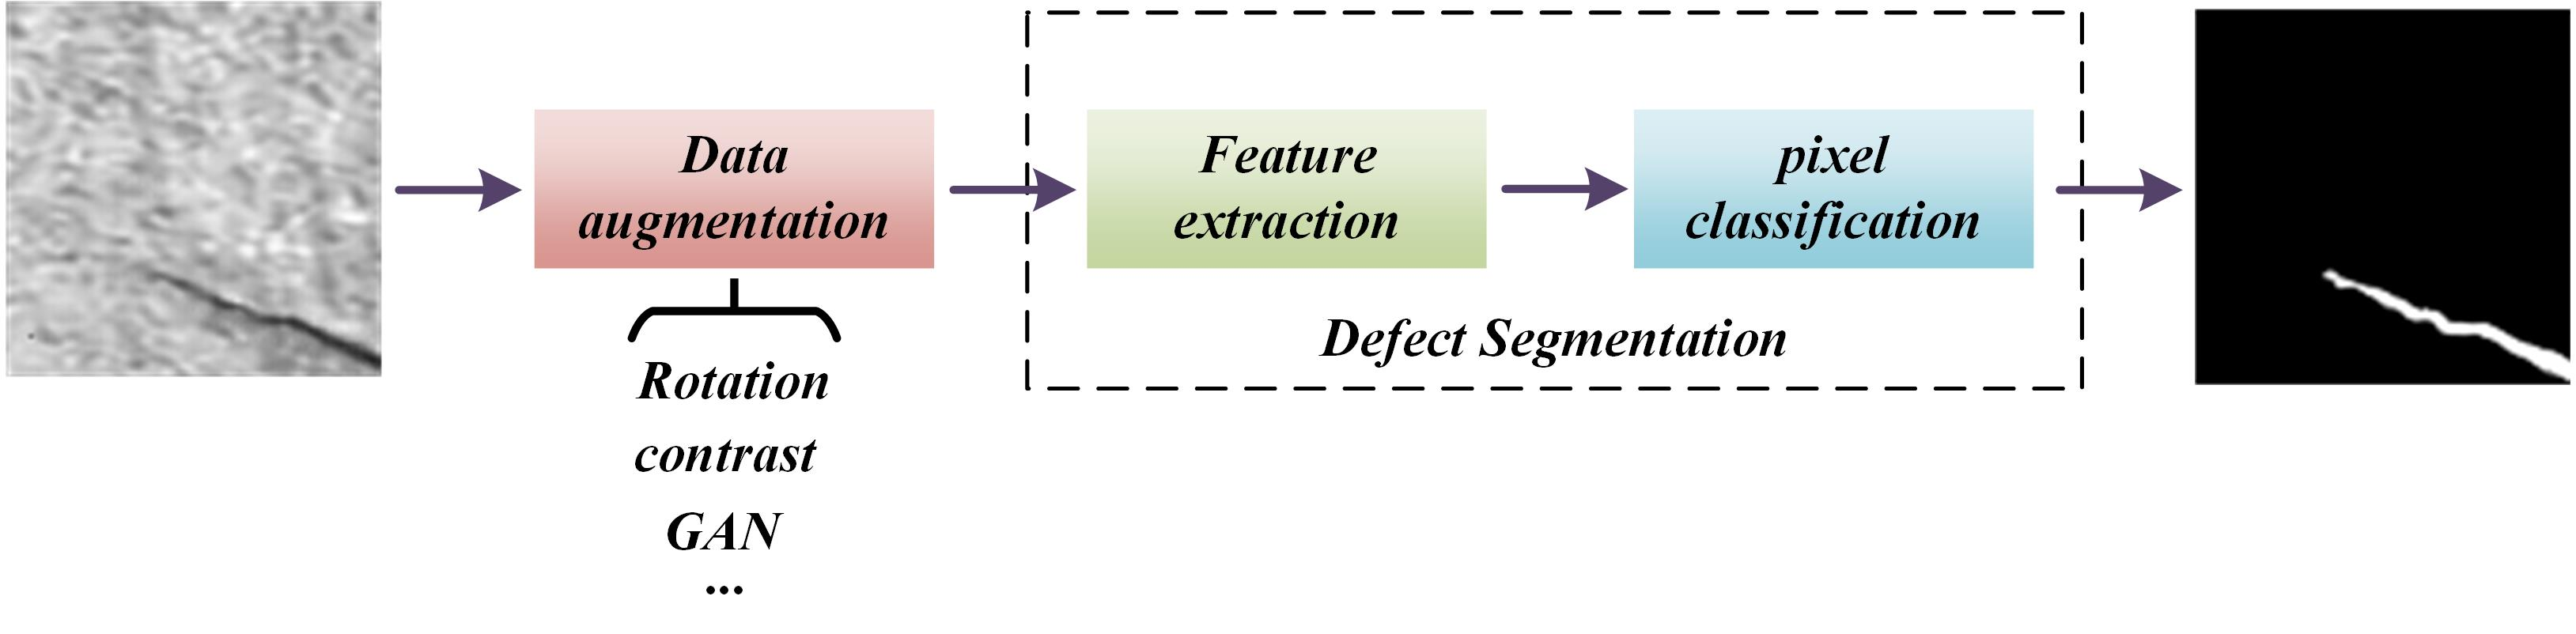
\includegraphics[width=4.5in]{fig1.jpg}
\caption{The pipeline of traditional data augmentation methods.}\label{fig:1.1}
\end{figure}

However, the purpose of data augmentation is to improve the performance of downstream CNN tasks. Therefore, the efficiency and effectiveness of data augmentation will be significantly improved based on the requirements of the given defect segmentation task.



This paper focuses on data augmentation for defect segmentation. Defect segmentation can predict the category for each pixel of the industrial image, so the accurate defect area can be obtained. Therefore, certain key features can be obtained by segmentation results, including position, shape, area, and contour, which are used to accurately judge the size and severity of defects. The mainstream CNN segmentation model includes a feature extractor and a pixel classifier. The confidence map shown in Fig. \ref{fig:1.2} can be obtained by the feature extractor, and this map represents the confidence values of the CNN for different defect regions. The CNN model has high confidence for the defect region in the yellow box, but it does not have sufficient confidence to detect the defect region in the red box in Fig. \ref{fig:1.2}.
Therefore, the proposed data augmentation approach shown in Fig. \ref{fig:1.3} improves the attention and ability of the CNN to detect low-confidence areas.
First, we pretrain the CNN model without data augmentation to reach a steady state. Then, the confidence map is obtained through the feature extractor. The defect regions with high confidence can be occluded, while those with low confidence can be maintained, forcing the CNN to focus on the defect regions that are difficult to detect. Finally, the confidence map can be updated to prevent overfitting after a period of training. Compared with other industrial data augmentation approaches, the proposed method does not need to train additional image generation models. In addition, it is simple to operate as a separate module that can be added to various existing defect segmentation models. Moreover, the proposed method fully utilizes the information contained in the existing dataset to meet the requirements of the CNN model. With the proposed data augmentation technique, the CNN model can significantly improve its defect segmentation accuracy and robustness, especially for defect regions with low confidence.


\begin{figure}
\centering
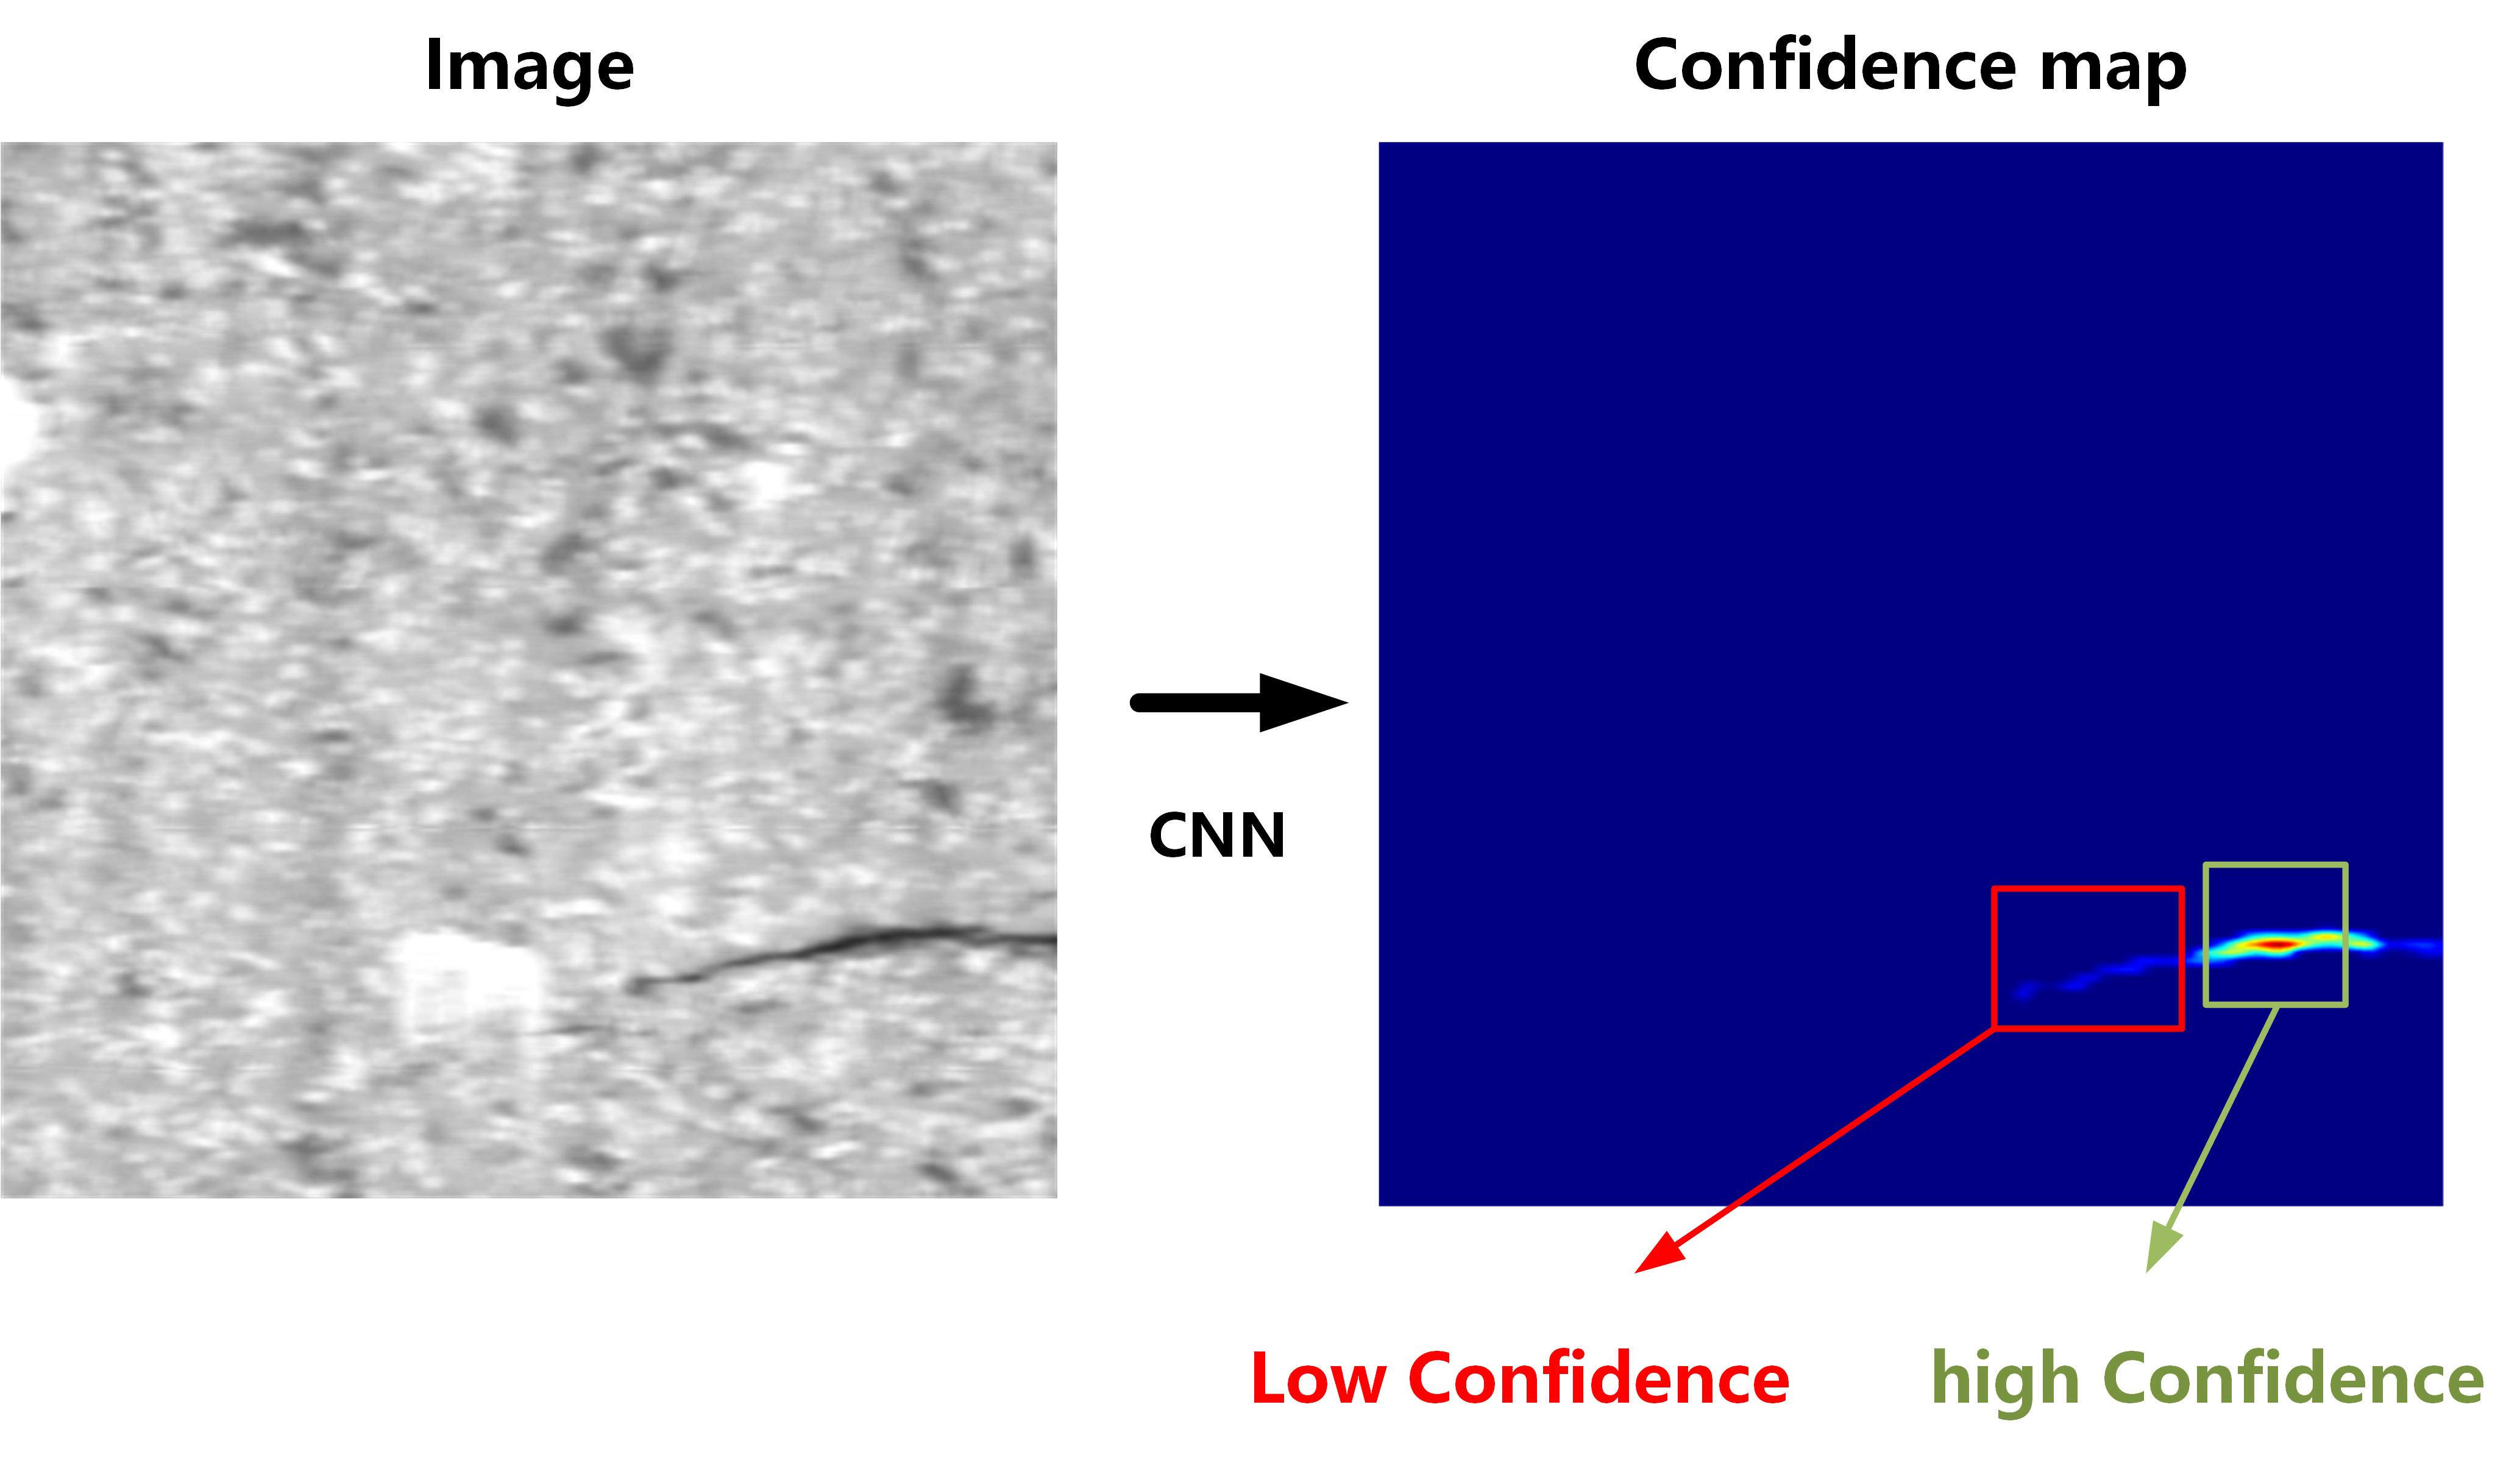
\includegraphics[width=3in]{fig2.jpg}
\caption{The confidence map for defect images obtained by a CNN.}\label{fig:1.2}
\end{figure}

\begin{figure}
\centering
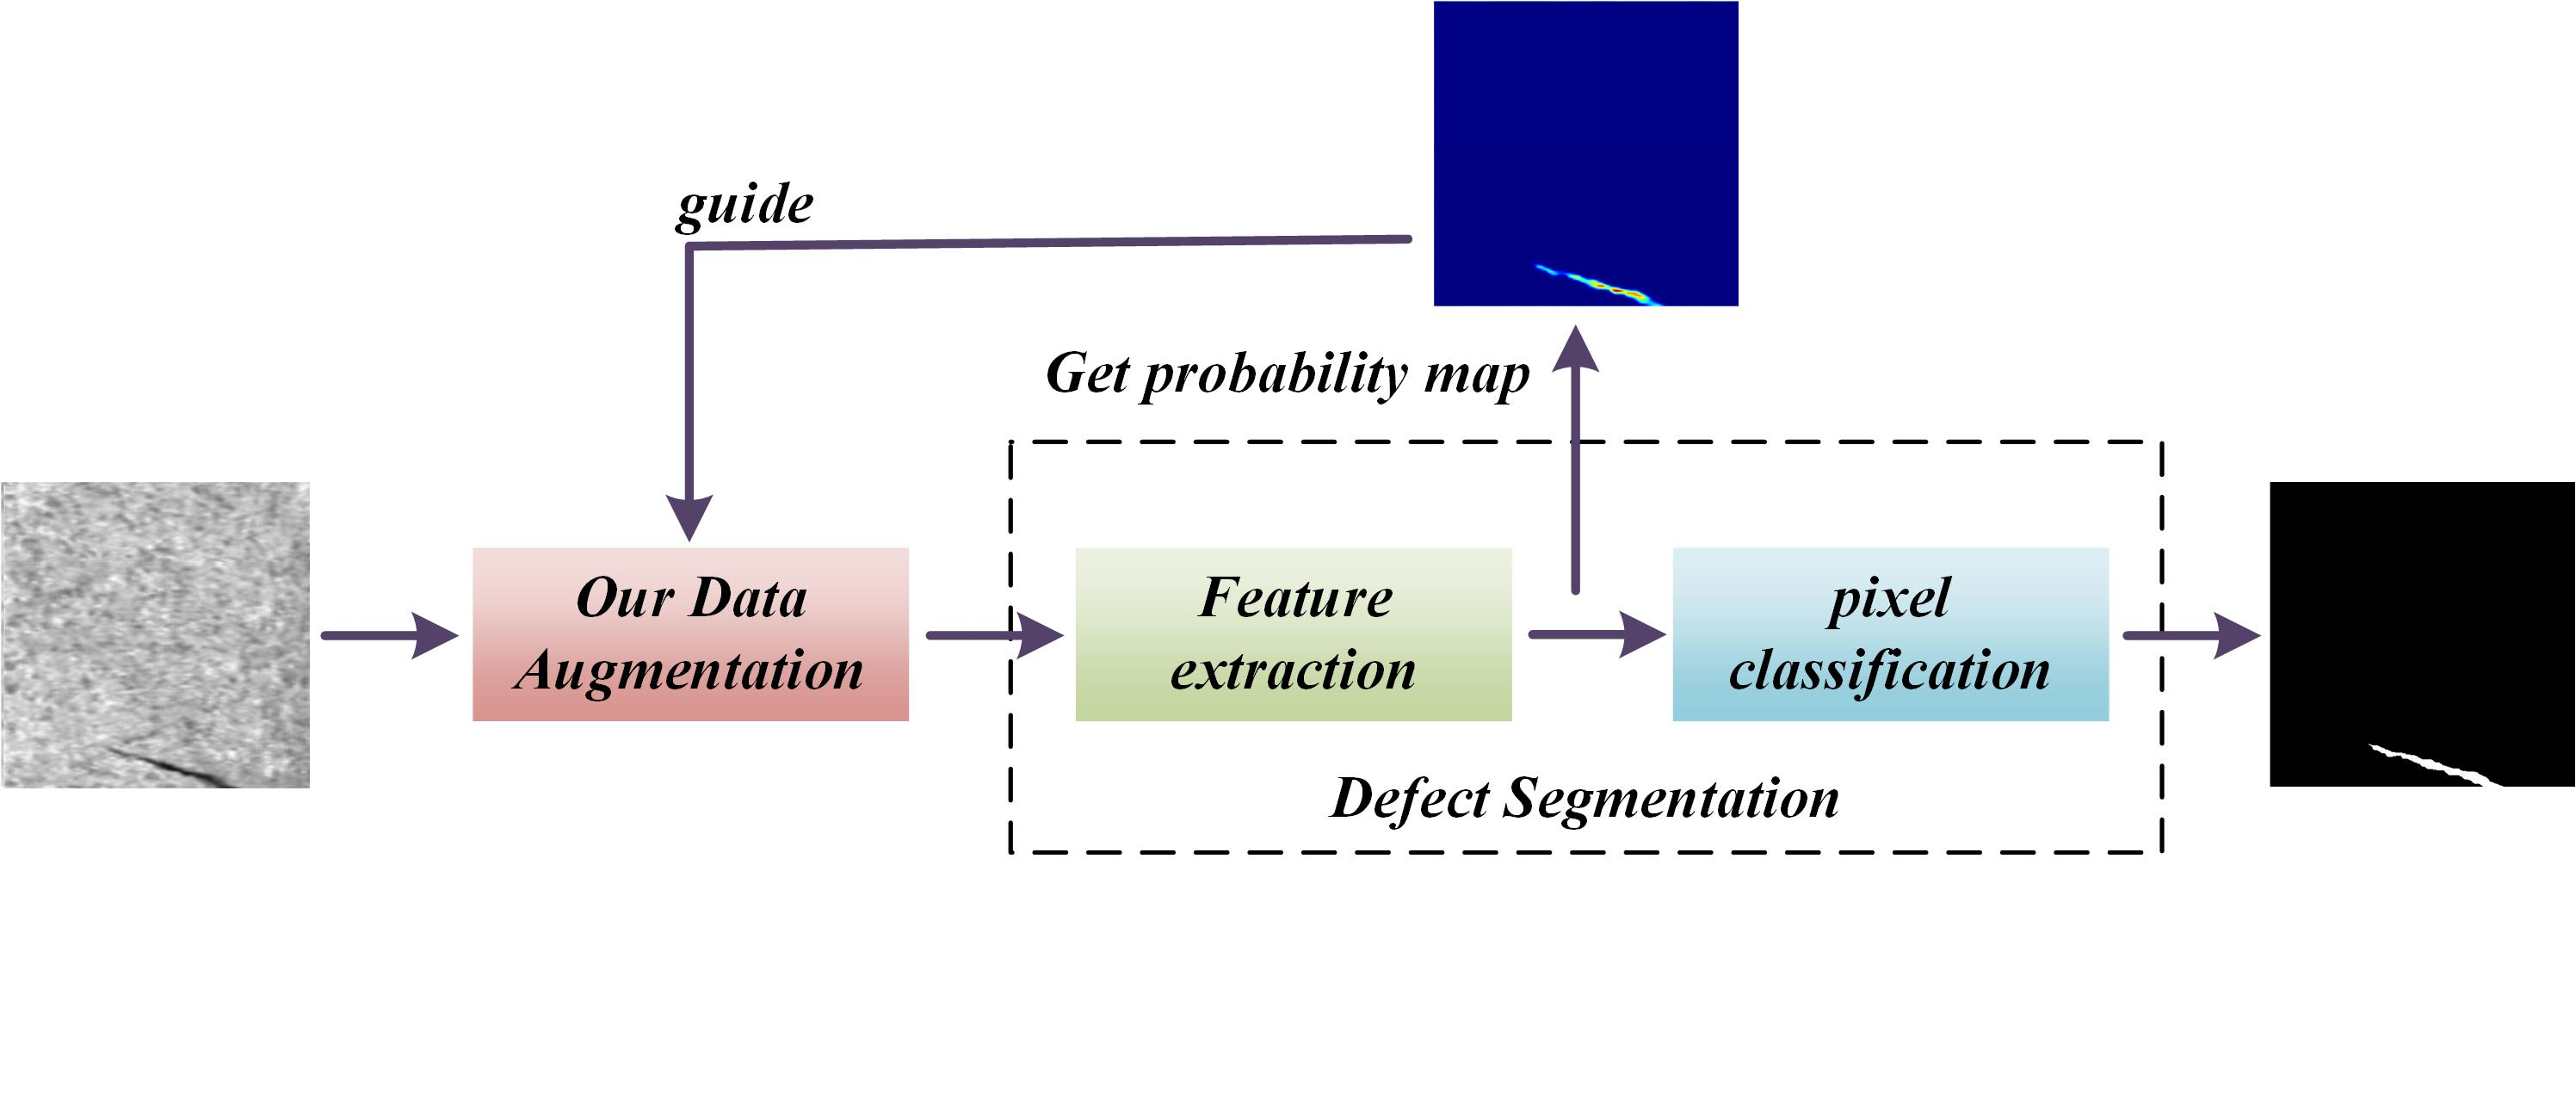
\includegraphics[width=4.5in]{fig3.jpg}
\caption{The proposed data augmentation method guided by a CNN.}\label{fig:1.3}
\end{figure}


The contributions can be summarized as follows:

\begin{enumerate}[1)]
\item We propose a simple, plug-and-play, and effective data augmentation method. Based on the confidence map obtained through pretraining, our approach can delete high-confidence defect regions to balance the attention paid by the defect segmentation model to high- and low-confidence regions.
\item We propose a novel defect augmentation approach that performs defect augmentation according to the requirements of the downstream defect segmentation model.
\item The proposed data augmentation method proves its effectiveness in terms of achieving improved defect segmentation accuracy and robustness and is highly generalizable to different existing segmentation frameworks.
\end{enumerate}


The remainder of the article is organized as follows. The related work on data augmentation methods and their applications in industrial vision is discussed in Section \ref{sec:rel}. Section \ref{sec:met} describes the proposed method in detail. Section \ref{sec:exp} presents the experimental results in comparison with those of different state-of-the-art methods. Finally, the conclusion and future work are summarized in Section \ref{sec:con}.


\section{The Related Work}\label{sec:rel}
\subsection{Data augmentation}
Data augmentation is an important way to solve data shortages and CNN model overfitting problems, and augmentation approaches can be divided into image conversion, image fusion, and image generation techniques.

Image conversion-based data augmentation methods include spatial transformations and color transformations.
\begin{enumerate}[1)]
\item Spatial transformations: flipping, translation, rotation, and so on.
\item Color transformations: noise injection, contrast, brightness transformation, and so on.
\end{enumerate}
Image conversions have become the basic operations in visual tasks involving various CNNs. For example, Muller \cite{muller2021trivialaugment} proposed TrivialAugment, which can sample an augmentation and a strength for each image and apply it.
Recently, information dropping has become a 
%Quality Control Editor: Please ensure that the intended meaning has been maintained in the following edit.
new and popular research topic 
for image conversion-based data augmentation.
Devries \cite{devries2017improved} proposed Cutout, which randomly uses a square mask as a regularization method to occlude a part of the input image.
HAS \cite{singh2017hide} divides an image into S*S blocks and randomly hides some image blocks.
Chen \cite{chen2020gridmask} proposed a structured occlusion-based augmentation method named GridMask that can delete regions with a set of spatially and uniformly distributed squares.

Image fusion combines the information derived from two or more images to form a new image.
Zhang \cite{zhang2017mixup} proposed Mixup, which performs weighted pixel interpolation with two images and their labels to obtain new samples.
Similar to Cutout, Cutmix \cite{yun2019cutmix} first occludes parts of one image and then fills the contents of another image with the corresponding position to achieve the fusion of the two images.
Hendrycks \cite{hendrycks2019augmix} proposed Augmix, which first uses geometric and color transformation to augment the input image and then fuses the augmented images.
TransMix \cite{chen2021transmix} fuses images and labels based on attention guidance for vision transformation tasks.
Ghiasi \cite{ghiasi2021simple} simply copy-pastes objects onto random images to augment instance segmentation datasets.

Image generation is mainly based on the variants of VAEs or GANs and generates a large number of images to increase the volume and diversity of datasets. It is widely used in different scenarios, such as pedestrian reidentification, road recognition, medical image detection and face recognition.
Zheng \cite{zheng2019joint} transformed pedestrian attributes and styles through a GAN to perform data augmentation and thus improved the accuracy of pedestrian reidentification.
Lin \cite{lin2020gan} improved the robustness of a road detection model by mapping road images obtained during the daytime and good weather to night, rainy and foggy weather conditions.
Uricar \cite{uricar2021let} proposed a dirty image GAN-based generation method to improve the diversity of the wide-angle fisheye camera dataset and significantly improve the autopilot accuracy of harsh environmental settings.
Choi \cite{choi2019self} presented a GAN-based data augmentation method to facilitate domain alignment between the images of game scenes and real scenes, reducing the difficulty and cost of data collection.
Zhang \cite{zhang2020robust} transformed license plate images produced by a template into a real scene through CycleGAN \cite{zhu2017unpaired} to improve the accuracy of license plate detection in unconstrained environments, such as reflection, blurring, and tilting.
Bissoto \cite{bissoto2021gan} synthesized samples indistinguishable from real images for skin lesion medical applications based on GANs, obtained favorable results from out-of-distribution test sets and achieved anonymization. 
Naghizadeh \cite{naghizadeh2021semantic} proposed a data augmentation method for biomedical and natural images, which can find and select the best policies for an autoencoder through a greedy search to generate cell images and masks.
Luo \cite{luo2021fa} presented a face augmentation generative adversarial network (FA-GAN) that designs a hierarchical disentanglement module to decouple the attributes of identity representation and can be applied to long-tail imbalanced data distributions.




\subsection{Industrial data augmentation}

Due to the characteristics of high yield rates and small numbers of abnormal samples in industrial sites, it is difficult to construct an industrial defect dataset that meets the requirements of deep learning for building CNN models with good generalization and robustness. Therefore, many scholars have attempted to design image augmentation methods for industrial defect detection  \cite{hsu2021multiple, schlosser2022improving}.

Many researchers have used geometric and color transformations of existing images to expand defect datasets. 
Paolo \cite{sassi2019smart} performed random rotations and flips to limit the decrease in performance for injector defect detection. 
Pan \cite{pan2021artificial} used traditional image transformation methods, such as rotation, cropping, flipping, and brightness and contrast adjustment, to augment CT defect images of wood.
Recently, with the rapid development of image generation technology, such as GANs, many researchers have tried to apply these approaches to industrial defect image generation \cite{jain2020synthetic,xuan2018multiview}.
Niu \cite{niu2020defect} proposed the surface defect-generation adversarial network (SD-GAN) based on a cycle-consistent loss and a dual adversarial loss to generate new defects with balanced image quality and diversity based on a large number of defect-free images. 
After generating defect images via Wasserstein GANs (WGANs), Le \cite{le2020learning} constructed a quality management model with fake and real images by transfer learning. 
Yang \cite{yang2021mask2defect} proposed a new data augmentation algorithm, named Mask2Defect, via prior knowledge infusion, which was able to generate a large volume of defects with different shapes, severities, scales, rotation angles, spatial locations, and part numbers. 
Yun \cite{yun2020automated} proposed a conditional CVAE (CCVAE) to generate images of each defect type in a single CVAE model for training a classification model. 
Liu \cite{liu2019multistage} proposed a multistage GAN to generate different defect patches given different texture backgrounds and then fused the generated defects at specific locations. 
Liu \cite{liu2021learning} proposed a novel stacked multimanifold autoencoder (S-MMAE) by introducing a new multimanifold regularization to offer a more comprehensive representation of original data, which can significantly increase prediction accuracy.
Based on a GAN and the Gaussian mixture model, Ren \cite{ren2022data} proposed a data augmentation method that can effectively increase the number of training samples and reduce distribution differences between training and test sets and thus obtain a significant improvement in sanitary-ceramic defect classification.
Li \cite{li2022eid} proposed a new augmentation model named extremely imbalanced data augmentation generative adversarial network (EID-GAN) with a new penalty function that guides the generator to learn the features of outliers, thus addressing the extremely imbalanced data augmentation problem.
Selecting the conditional GAN and geometrical transformation techniques, Liu \cite{liu2021defect} proposed a data augmentation method to improve the diversity and realism of synthetic defects in laser line scan sensor images.
Tang \cite{tang2022cascaded} proposed a data generation methodology based on homography transformation and image fusion that can generate tobacco pack images with foreign objects.
The above defect augmentation methods can significantly improve the performance of the downstream task defect detection model. However, they require a certain amount of data to build a generative model and are independent of downstream task defect detection.

\section{Methodology}\label{sec:met}
\subsection{The pipeline of the proposed method}\label{sec:In}

\begin{figure}
\centering
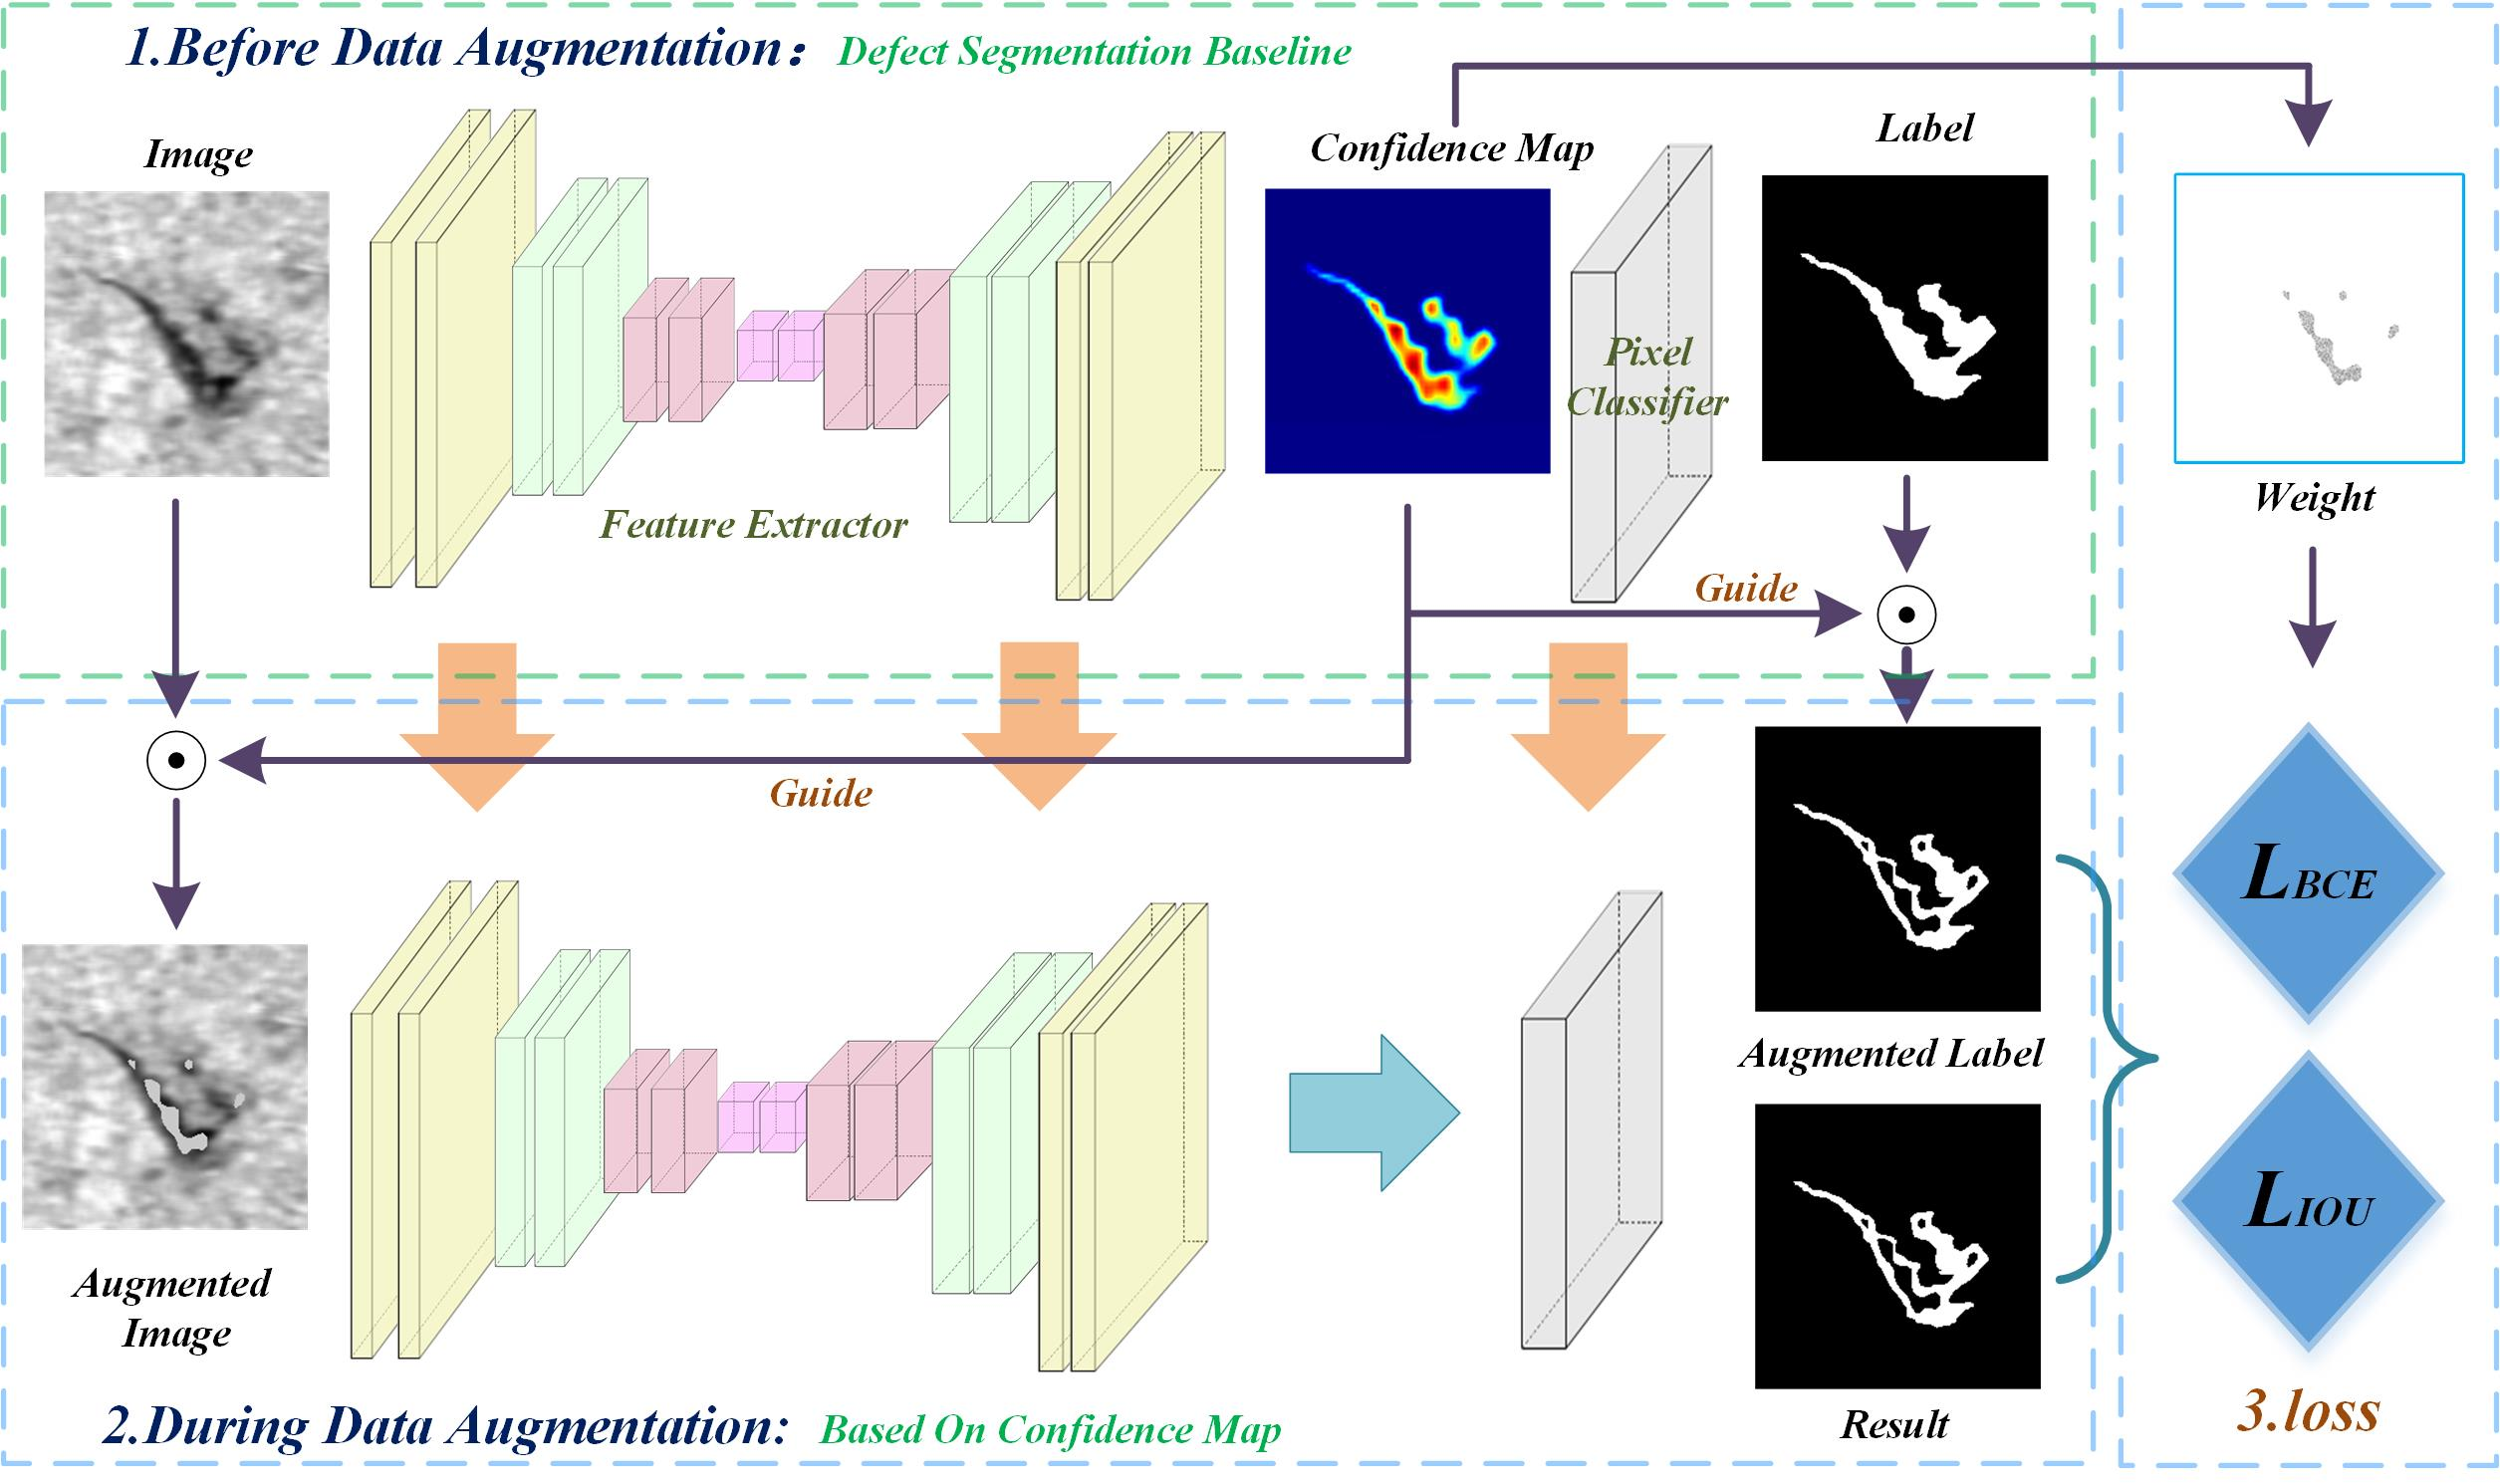
\includegraphics[width=4.5in]{fig4.jpg}
\caption{The pipeline of the proposed data augmentation method.}\label{fig:3.1}
\end{figure}

In this section, we propose a new data augmentation method based on the requirements of downstream CNN-based defect segmentation tasks shown in Fig. \ref{fig:3.1}, which contains the following modules.
\begin{enumerate}[1)]
\item \textbf{Baseline defect segmentation module}: This module includes two submodules: feature extractor and pixel classifier. The feature extractor can be used to obtain confidence maps for defect images in training sets.
\item \textbf{Data augmentation module based on a CNN}: The information-dropping data augmentation method is performed according to the obtained confidence maps.
\item \textbf{Loss function module}: This module can be divided into normal loss functions before data augmentation and weight-guided loss functions during data augmentation.
\end{enumerate}
The proposed data augmentation strategy is a simple and plug-and-play method that can be directly applied to existing CNN-based defect segmentation algorithms during training. Therefore, the training process of the proposed method can be divided into a normal mode and an augmentation mode. The normal mode used in the early stage trains the defect segmentation model without data augmentation. Until the model reaches a steady state with a stable confidence map, we use the augmentation mode to further improve the performance of the CNN model. 

\subsection{The baselines for CNN defect segmentation}\label{sec:In}
Existing defect segmentation models generally use popular image segmentation algorithms, such as UNet \cite{ronneberger2015u}, DeepLab \cite{chen2018deeplab:}, and fully convolutional networks (FCNs) \cite{long2015fully}, which are widely utilized in various defect segmentation scenarios. The defect segmentation model $f_s$ can generally be divided into feature extractor and pixel classifier modules. 

\textbf{Feature extractor module $f_{fe}$} : consists of different network modules, such as the inception module \cite{szegedy2016rethinking}, resblock module \cite{he2016deep}, and dense module \cite{huang2017densely}, which are composed of different base layers, such as convolution, pooling, and normalization layers. It mainly extracts the features of input image $X$ in a layer-by-layer manner to obtain confidence maps $P$.
\begin{equation}
\centering
\begin{split}
P = f_{fe}(X)
\end{split}
\end{equation}
\textbf{Pixel classifier module $f_{pc}$}: consists of Sigmoid or Softmax layers. It can determine image segmentation results $R$ based on the obtained confidence map $P$. 
\begin{equation}
\centering
\begin{split}
R = f_{pc}(P)
\end{split}
\end{equation}
The value of the confidence map indicates the confidence level of the CNN model regarding whether it considers the corresponding area to be a defect region. The proposed data augmentation method is constructed based on the guidance of the confidence map.

\subsection{Information dropping-based data augmentation}\label{sec:In}

Information dropping is a popular data augmentation strategy that removes parts of an image to improve the perception of a CNN model with respect to originally insensitive information, thereby increasing the robustness of the model. This strategy has been widely considered to be effective in many visual scenes. Therefore, the proposed method also adopts the strategy of information dropping to perform data augmentation. Mainstream information dropping approaches are mainly divided into three categories.

\begin{enumerate}[1)]
\item Randomly deleting a rectangular area of an image (e.g., Cutout \cite{devries2017improved}).
\item Dividing the image into S*S image blocks and randomly removing some image blocks (e.g., HAS \cite{singh2017hide}).
\item Building masks with noncontiguous structures and deleting image regions by multiplying the masks (e.g., GridMask \cite{chen2020gridmask}).
\end{enumerate}

However, most of the above strategies, especially Cutout\cite{devries2017improved} and HAS \cite{singh2017hide}, randomly produce invalid data augmentation results, such as those with excessive dropping and undeleted defective areas. On the one hand, excessive dropping (the red box in Fig. \ref{fig:3.3.1}) deletes most of the context of the defect feature to change the image attributes. This results in negative optimization for the subsequent defect detection step. On the other hand, the nondeletion of defect regions (the blue box in Fig. \ref{fig:3.3.1}) has a negligible impact on the robustness of a CNN model. Moreover, some of the above methods, such as GridMask, are based on set rules, such as discontinuous grids, which can effectively prevent excessive dropping and the nondeletion of defects. However, they cannot effectively guarantee that the deleted image content is sensitive or ignored by the CNN model.

To improve the effectiveness of information dropping for defect images, the proposed method constructs a defect dropping strategy based on the requirements of the utilized CNN model.

\begin{figure}
\centering
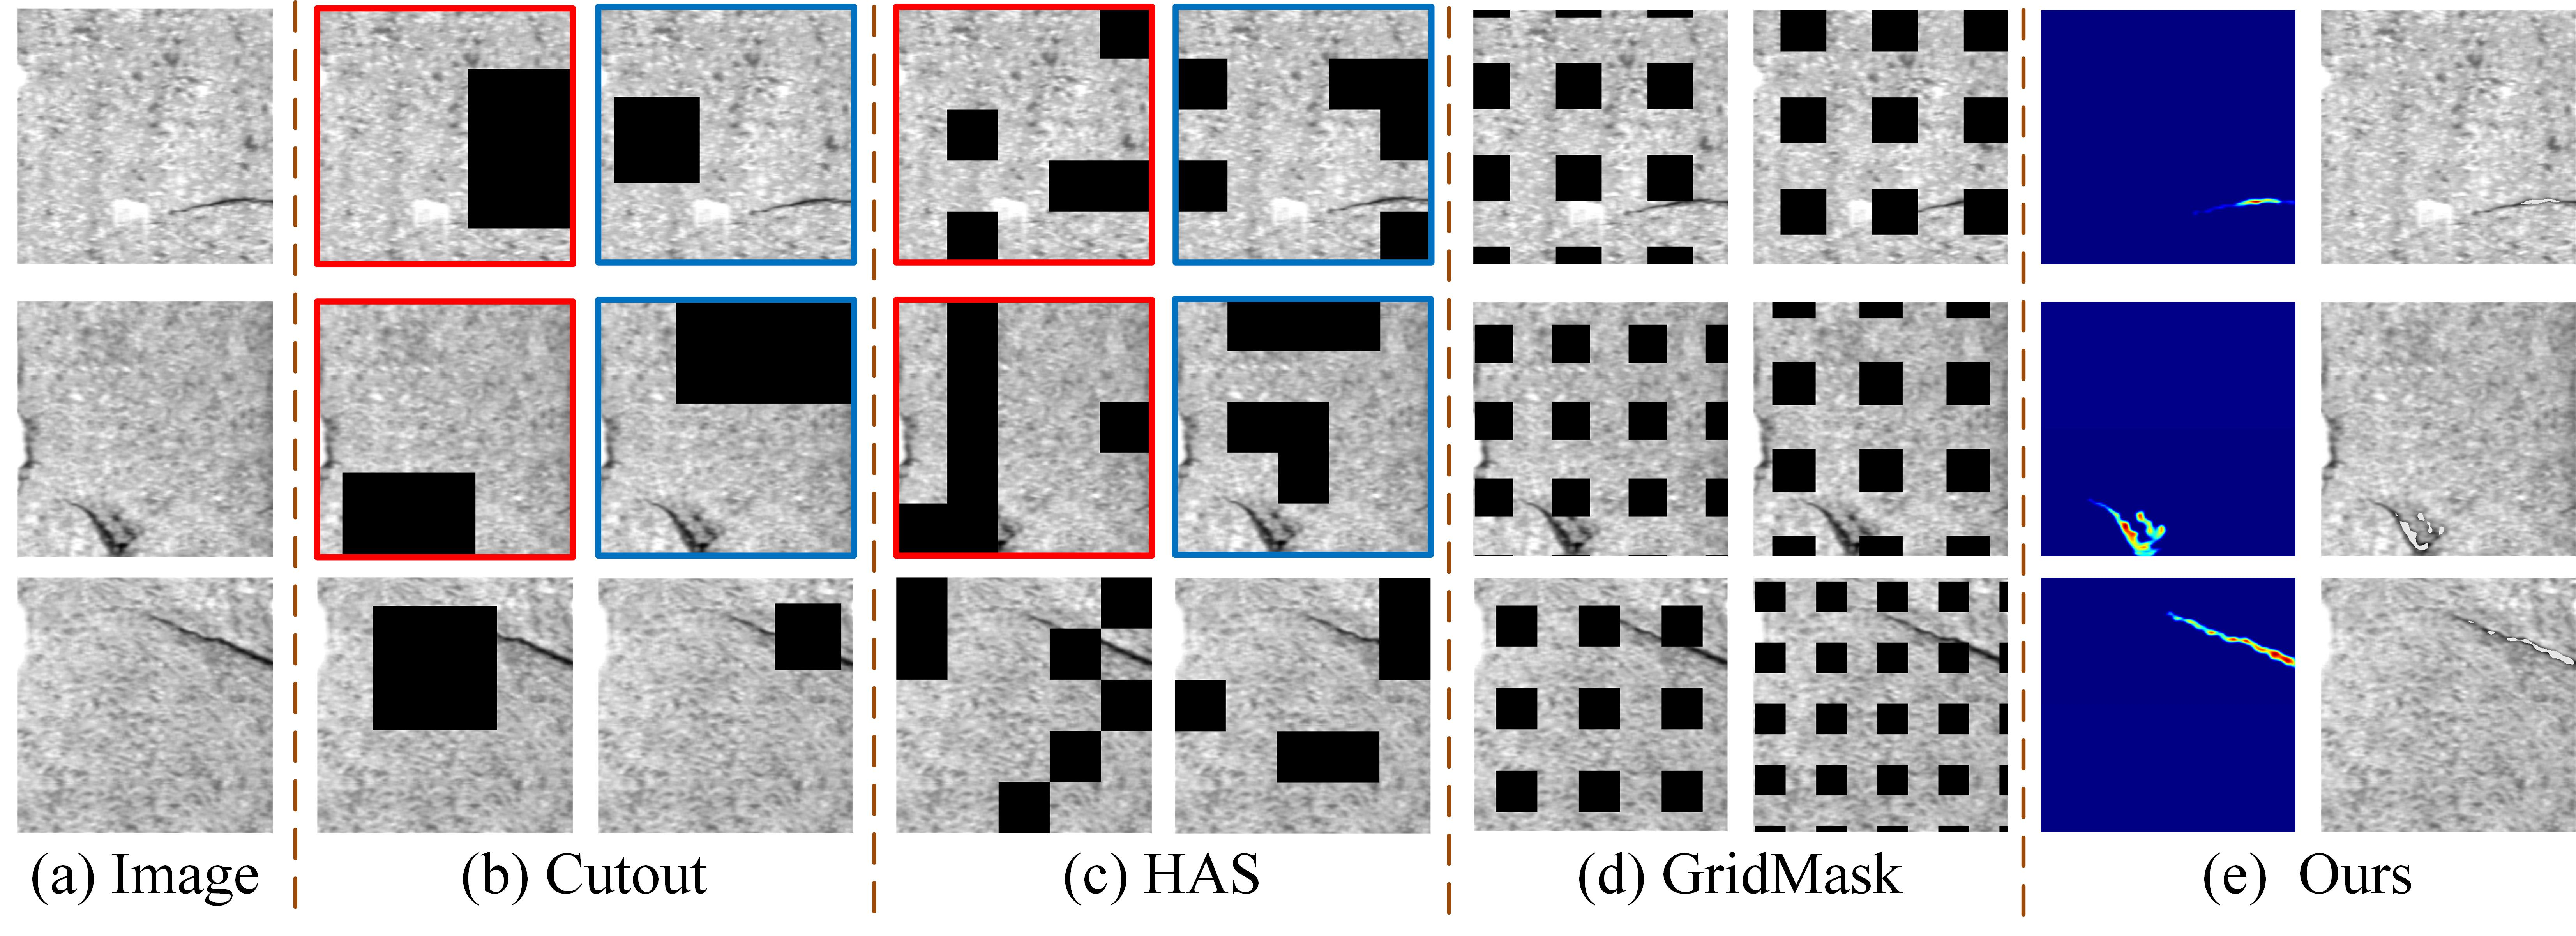
\includegraphics[width=4.5in]{fig5.jpg}
\caption{A comparison of different information dropping data augmentation strategies.}\label{fig:3.3.1}
\end{figure}


\subsection{Data augmentation based on CNN}\label{sec:In}

Due to the inconsistencies among the characteristics of different areas within a defect, such as grayscale, texture, and position attributes, the detection difficulty levels of different defect areas are different. It is difficult for humans to accurately analyze the detection difficulty levels of different specific defect areas to set a rule for data augmentation. Since the purpose of data augmentation is to improve the ability to complete the downstream CNN tasks, the confidence map obtained by the employed CNN model can be used as a guide for its detection capability of different defect areas. Defect areas with high confidence are considered detectable by the CNN model as easy-to-detect defect regions. Conversely, low-confidence regions can be considered difficult-to-detect defect regions.

Since the purpose of information dropping-based data augmentation is to improve a CNN model's perception of insensitive information, our augmentation scheme is to delete the defect areas that are easy to detect with the CNN model and improve the model's attention to the difficult-to-detect defect areas. The specific steps are as follows.

\begin{enumerate}[1)]
\item Based on the pretraining of the CNN model, a confidence map $P$ is obtained for each image in the training set. The closer the color of the confidence map is to red, the higher the confidence is and the easier the associated area is to detect. The confidence map can be used as a guide for data augmentation.

\item Data augmentation module $f_d$ includes $f_{dx}$ for input image $X$ and $f_{dy}$ for label $Y$. A threshold T is randomly chosen.
\begin{equation}
\centering
f_d = <f_{dx}, f_{dy}>
\end{equation}

For $f_{dx}$, the confidence values $p_i$ are above the threshold $T$, and the corresponding areas in image $X$ are occluded with the average value of the background. The regions of image $X$ with confidence values $p_i$ below the threshold $T$ are retained. $X_{aug}$ represents the augmented image

\begin{equation}
\centering
X_{aug} = f_{dx}(X) = \left\{
\begin{aligned}
mean(X[Y=0]), &~~p_i > T \\
X~~~~~~~,&~~p_i < T \\
\end{aligned}
\right.
\label{eq:fdx}
\end{equation}

For $f_{dy}$, the areas with the label $Y$ above $T$ are removed and that below threshold $T$ is retained. $Y_{aug}$ represents the augmented label.

\begin{equation}
\centering
Y_{aug} = f_{dy}(Y) = \left\{
\begin{aligned}
0, &~~p_i > T \\
Y, &~~p_i < T \\
\end{aligned}
\right.
\label{eq:fdy}
\end{equation}
\item The retention rate of defect area $\eta$ is the proportion of the retained defect area in image $X_{aug}$ in the entire defect area of image $X$, defined as formula (\ref{eq:3.4.5}). We choose the range of $\eta$ to be (0.2, 0.8).

\begin{equation}
\centering
\eta = \frac{X_{aug} (Y_{aug} = 1)}{X (Y = 1)}
\label{eq:3.4.5}
\end{equation}

\item Due to the long-term training with an invariant confidence map, high-confidence regions at fixed locations are removed with high probability. Therefore, the model pays more attention to low-confidence regions. However, conducting iterative training for a long time can cause overfitting, resulting in the transformation of the confidence maps of defect images. Therefore, after the CNN model iterates for a period of time, the guiding confidence map is updated according to the training progress. In this work, we set the epoch of the update cycle $E_{uc}$ to 150 epochs as follows: 

When epoch $E != n*150$, we train the segmentation model based on the data augmentation module $f_{d}$.
\begin{equation}
\centering
\begin{split}
f_{dy}(Y_{aug}) = f_{pc}(f_{fe}(f_{dx}(X_{aug})))~~~with~~~E~!= n*150, n \in (1,2,3,...)
\end{split}
\end{equation}

When epoch $E = n*150$, we update the guiding confidence maps $P$:

\begin{equation}
\centering
\begin{split}
P_{new} = f_{fe}(X)~~~with~~~E~= n*150, n \in (1,2,3,...)
\end{split}
\end{equation}

The segmentation model is trained based on the new confidence map $P_{new}$ until the next update for $P$.

\end{enumerate}

\subsection{Loss function}\label{sec:loss}
To iterate and optimize the network described above, it is necessary to construct a loss function. The loss function is divided into losses for two stages: before and during data augmentation.

\textbf{Before data augmentation} The losses include the binary cross-entropy (BCE) loss and intersection-over-union (IOU) loss, which are very common and mainstream for defect segmentation.
\begin{enumerate}[]
\item The BCE loss measures the difference between the predicted class and the ground truth of each pixel, handling binary classification for each pixel.
\begin{equation}
\centering
\begin{split}
Loss_{BCE}(R,Y) = - (y_i\lg r_i + (1-y_i)\lg (1-r_i) )
\label{eq:3.3.8}
\end{split}
\end{equation}
$X$ represents the predicted map, and $Y$ represents the ground truth. $x_i$ and $y_i$ represent the predicted and true values of each pixel, respectively.

\item The IOU indicates the ratio between the intersection and union of $X$ and $Y$. The IOU loss measures how close the IOU is to 1. 
\begin{equation}
\centering
\begin{split}
Loss_{IOU}(R,Y) = 1 - \frac{R \cap Y}{R \cup Y}
\label{eq:3.3.8}
\end{split}
\end{equation}
\end{enumerate}

\begin{table}
\begin{center}
\begin{tabular}{ccccccc}
\toprule
\leftline{\textbf{Algorithm 1}} \\
\leftline{The training process of the CNN with the proposed data augmentation approach.}\\
\midrule
\leftline{\textbf{Input: } Image $X$ and its label $Y$} \\
\leftline{\textbf{Output: } Predicted result $R$} \\
\leftline{\textbf{Initialize} the defect segmentation network $f_s$} \\
\leftline{~~~~~~~~~~~~~~~Contains a feature extractor $f_{fe}$ and a pixel classifier $f_{pc}$} \\
\leftline{\textbf{while} epoch$\le$300 (Before data augmentation):} \\
\leftline{~~~~\textbf{for} i=1,...,n, \textbf{do}} \\
\leftline{~~~~~~~~Obtain the predicted result $R = f_{pc}(f_{fe}(X))$} \\
\leftline{~~~~~~~~Calculate the loss $Loss_{total} (R, Y)$} \\
\leftline{~~~~~~~~Backpropagate the $Loss_{total}$, update the segmentation network $f_s$} \\
\leftline{~~~~\textbf{end for}} \\
\leftline{\textbf{end while}} \\
\leftline{\textbf{While} epoch $>$ 300 (during data augmentation):} \\
\leftline{~~~~\textbf{If} epoch$\%$150 = 0:} \\
\leftline{~~~~~~~~Obtain or update the confidence map $P=f_{fe}(X)$} \\
\leftline{~~~~\textbf{for} i=1,...,n, \textbf{do}} \\
\leftline{~~~~~~~~Perform data augmentation for $X$ to generate $X_{aug}$ using (\ref{eq:fdx}) } \\
\leftline{~~~~~~~~Perform data augmentation for $Y$ to generate $Y_{aug}$ using (\ref{eq:fdy}) } \\
\leftline{~~~~~~~~Obtain the predicted result $ R= f_{pc}(f_{fe}(X_{aug}))$} \\
\leftline{~~~~~~~~Calculate the loss $Loss_{total} (R, Y_{aug})$} \\
\leftline{~~~~~~~~Backpropagate the $Loss_{total}$, update the segmentation network $f_s$} \\
\leftline{~~~~\textbf{end for}} \\
\leftline{\textbf{end while}} \\
\leftline{\textbf{Return:} R} \\
\botrule

\end{tabular}
\label{Algorithm 1}
\end{center}
\end{table}

\textbf{During data augmentation} Since the high-confidence regions of a defect image are occluded, we set lower weights for those regions. 
We construct a loss weight map $V$. The weight is set to a random value within the range of 0.5-1 for the filled region, and the weight is set to 1 for the original region.
\begin{equation}
\centering
V =\left\{
\begin{aligned}
rand(0.5,1), &~~p_i > T \\
1~~~~~~~,&~~p_i < T \\
\end{aligned}
\right.
\end{equation}
The loss functions are constructed based on the weight map $V$ to guide the training of the CNN model. The BCE and IOU losses based on weight are shown as follows:

\begin{equation}
\centering
\begin{split}
Loss_{BCE}(R,Y,V) = - v_i * (y_i\lg r_i + (1-y_i)\lg (1-r_i) )
\label{eq:3.3.8}
\end{split}
\end{equation}

\begin{equation}
\centering
\begin{split}
Loss_{IOU}(R,Y,V) = 1 - \frac{(R \cdot V)\cap (Y \cdot V)}{(R \cdot V) \cup (Y \cdot V)}
\label{eq:3.3.8}
\end{split}
\end{equation}
The total loss is shown as follows:
\begin{equation}
\centering
\begin{split}
Loss_{total} = Loss_{BCE} + \lambda Loss_{IOU} 
\label{eq:3.3.8}
\end{split}
\end{equation}

To more clearly represent the training process of this method, the pseudocode is shown in Algorithm 1.


\section{Experiments}\label{sec:exp}
\subsection{Setup}\label{sec:exp.1}
\subsubsection{Dataset}\label{sec:exp.1.1}
The industrial Kolektor surface defect (KSD) segmentation dataset \cite{tabernik2020segmentation} is chosen to verify the proposed data augmentation method. In order to simulate the situation that defects with weak intensity are difficult to collect in the industrial field, more defects with normal intensity are allocated in the training set $D_{tr}$ and more weak defects are allocated in the test set $D_{te}$. Since the image size in KSD is 500x1250, we cut each image into blocks of size 500x500 by using a stride of 150 pixels. The training set consists of 150 images, and the test set consists of 60 images. Fig. \ref{fig:4.1.sample} shows defect samples in the test and training sets.




\begin{figure*}
     \setlength{\abovecaptionskip}{0.cm}
     \setlength{\belowcaptionskip}{-0.cm}
	\centering
\scalebox{0.9}{
\begin{tabular}{p{1.6cm}p{1.6cm}p{1.6cm}p{0.5cm}p{1.6cm}p{1.6cm}p{1.6cm}}

			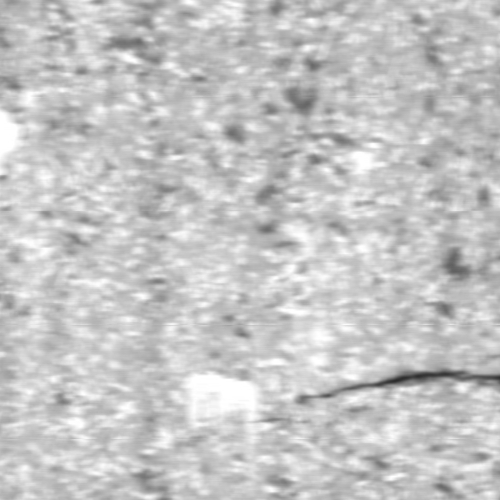
\includegraphics[width=0.7in]{fig6-train1.png}&
 			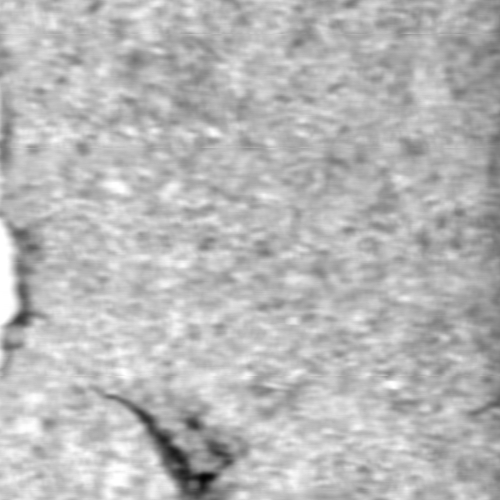
\includegraphics[width=0.7in]{fig6-train2.png}&
			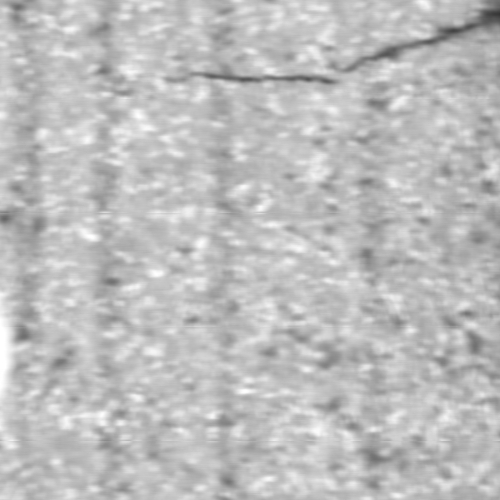
\includegraphics[width=0.7in]{fig6-train3.png}&&  
			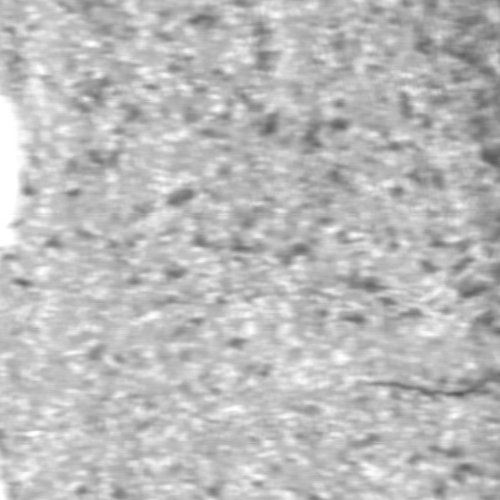
\includegraphics[width=0.7in]{fig6-test1.png}&
 			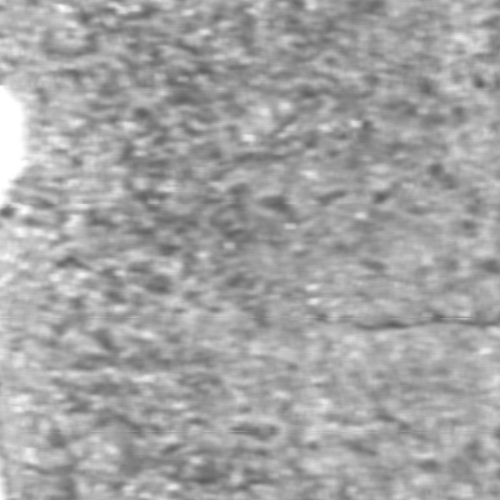
\includegraphics[width=0.7in]{fig6-test2.png}&
			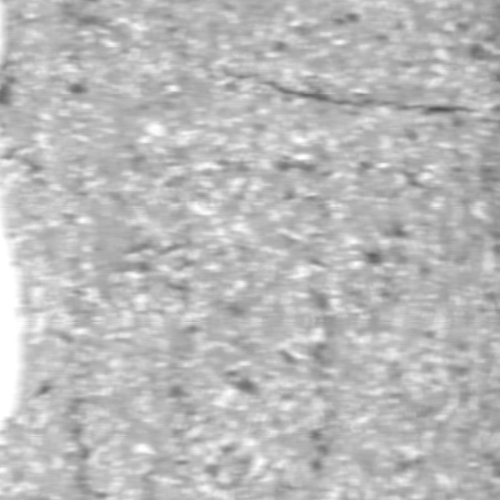
\includegraphics[width=0.7in]{fig6-test3.png} \\
\multicolumn{3}{c}{(a) training set}&&\multicolumn{3}{c}{(b) test set}
\end{tabular}}
	\centering
	\caption{The defect samples of training and test set for KSD dataset. (a) Training set. (b) Test set. }
	\label{fig:4.1.sample}
\end{figure*}


\subsubsection{Evaluation indicators}\label{sec:exp.1.2}
The IOU and PA are selected as the evaluation indicators ($EI$) of segmentation performance, as they are universal and widely used in different segmentation scenarios.
The IOU represents the ratio between the intersection and union of the predicted results and the ground truth.
PA represents the proportion of correctly classified pixels to total pixels.
\begin{equation}
\centering
\setlength{\abovedisplayskip}{3pt}
\setlength{\belowdisplayskip}{3pt}
\begin{split}
PA &= \frac{\sum_{i=0}^{k}P_{ii}}{\sum_{i=0}^{k}\sum_{j=0}^{k}P_{ij}}
\label{eq:3.3.8}
\end{split}
\end{equation}
\begin{equation}
\centering
\setlength{\abovedisplayskip}{3pt}
\setlength{\belowdisplayskip}{3pt}
\begin{split}
IOU &= \frac{\sum_{i=0}^{k}P_{ii}}{\sum_{j=0}^{k}P_{ij}+\sum_{j=0}^{k}P_{ji} - \sum_{i=0}^{k}P_{ii}}
\label{eq:3.3.8}
\end{split}
\end{equation}
\subsubsection{Implementation details}\label{sec:exp.1.2}
The experiment is run using an NVIDIA RTX 1080 graphics processing unit (GPU). All experiments are implemented on a deep learning framework consisting of PyTorch 1.0 and NumPy.
Except for the data augmentation module, all models are set with the same parameters. The optimizer is Adam \cite{kingma2014adam} with a learning rate of 0.001, and the number of training epochs is 2000.

\subsection{Confidence map analysis and chosen hyperparameters}\label{sec:exp.3}

\begin{figure*}
     \setlength{\abovecaptionskip}{0.cm}
     \setlength{\belowcaptionskip}{-0.cm}
	\centering
\scalebox{0.9}{
\begin{tabular}{p{1.2cm}p{1.2cm}p{1.2cm}p{1.2cm}p{1.2cm}p{1.2cm}p{1.2cm}p{1.2cm}}

    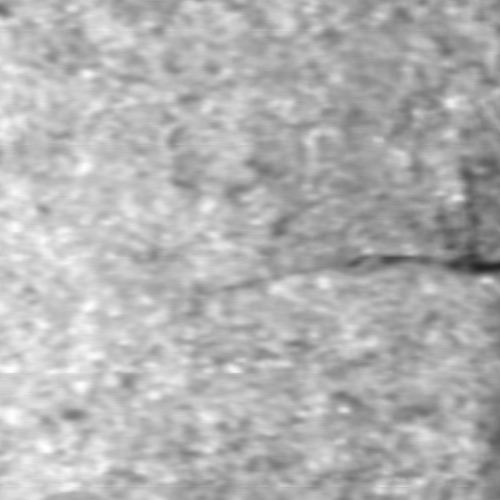
\includegraphics[width=0.6in]{fig7-1.png}&
    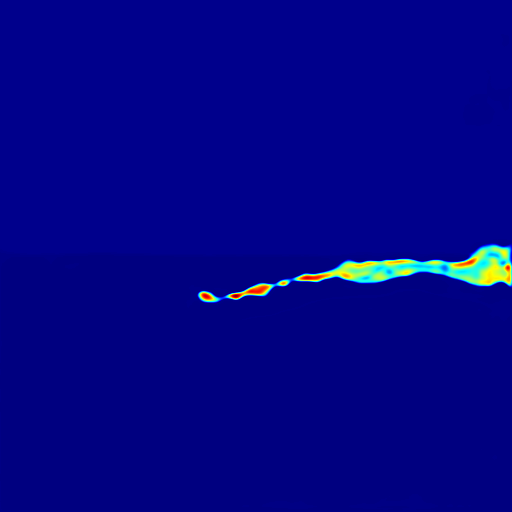
\includegraphics[width=0.6in]{fig7-1-0.png}&
    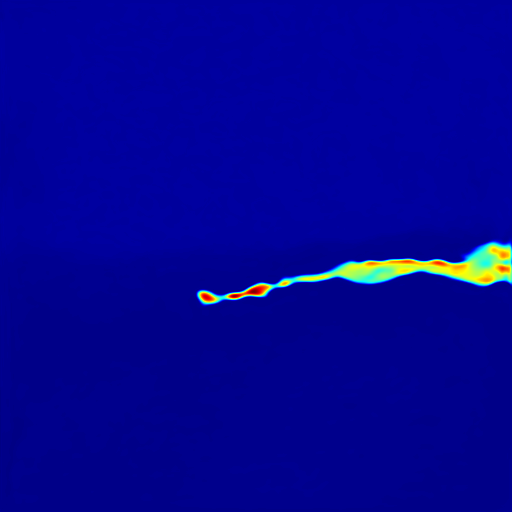
\includegraphics[width=0.6in]{fig7-1-50.png}&
    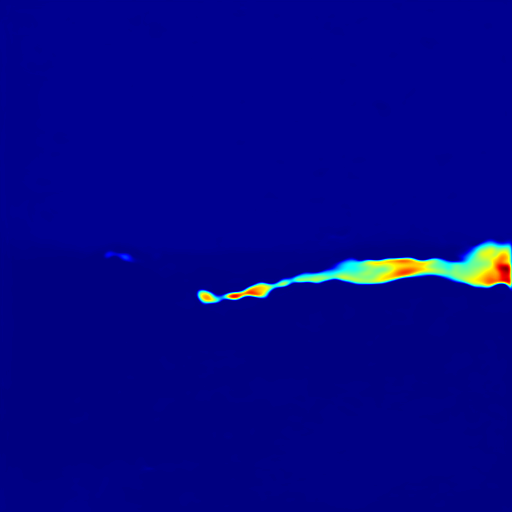
\includegraphics[width=0.6in]{fig7-1-100.png}&
    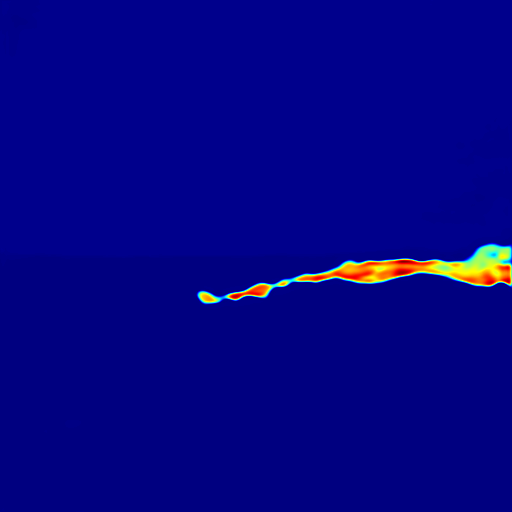
\includegraphics[width=0.6in]{fig7-1-150.png}&
    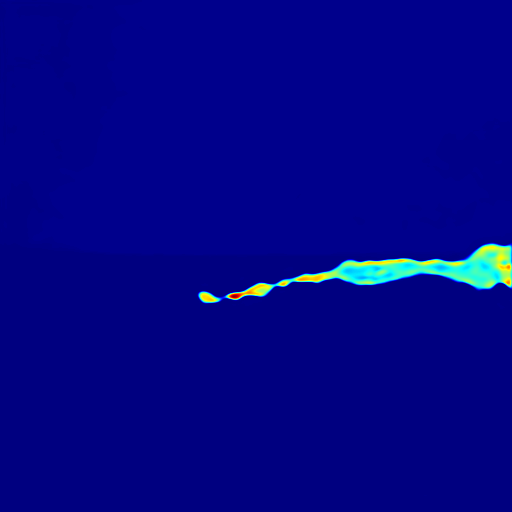
\includegraphics[width=0.6in]{fig7-1-200.png}&
    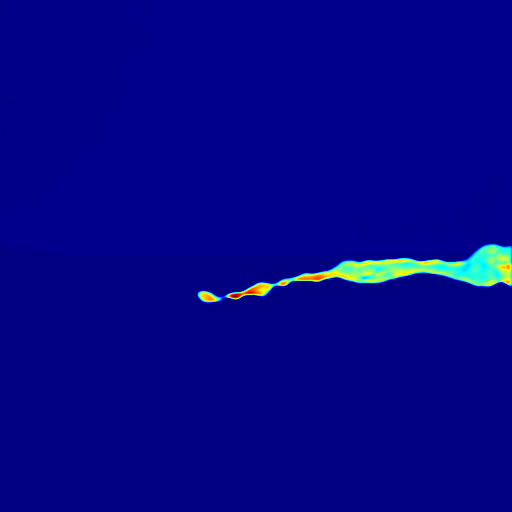
\includegraphics[width=0.6in]{fig7-1-250.png}&
    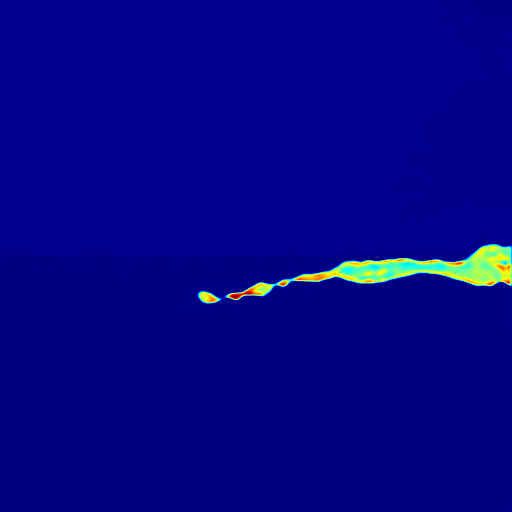
\includegraphics[width=0.6in]{fig7-1-300.png}\\

    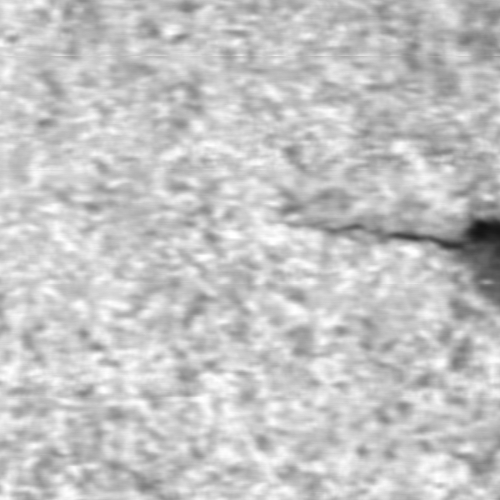
\includegraphics[width=0.6in]{fig7-2.png}&
    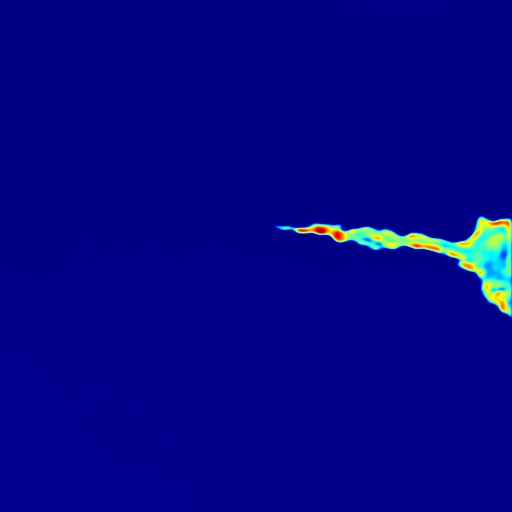
\includegraphics[width=0.6in]{fig7-2-0.png}&
    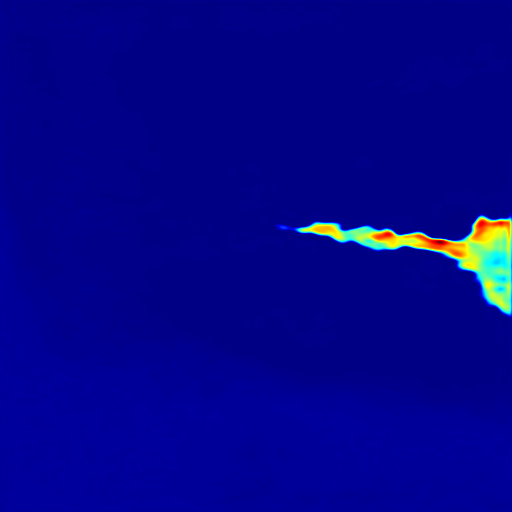
\includegraphics[width=0.6in]{fig7-2-50.png}&
    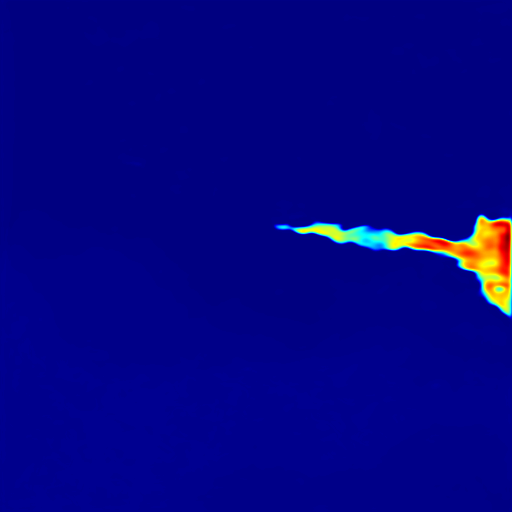
\includegraphics[width=0.6in]{fig7-2-100.png}&
    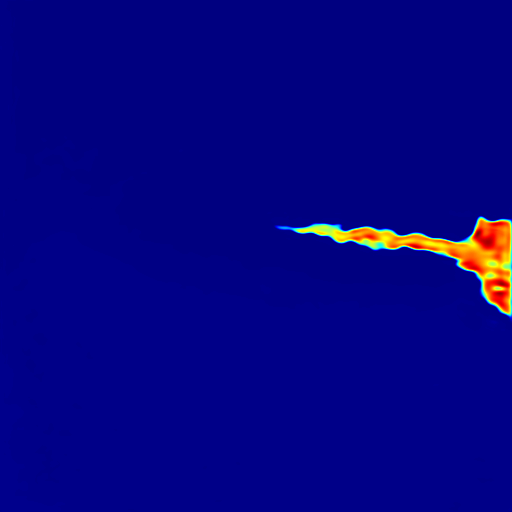
\includegraphics[width=0.6in]{fig7-2-150.png}&
    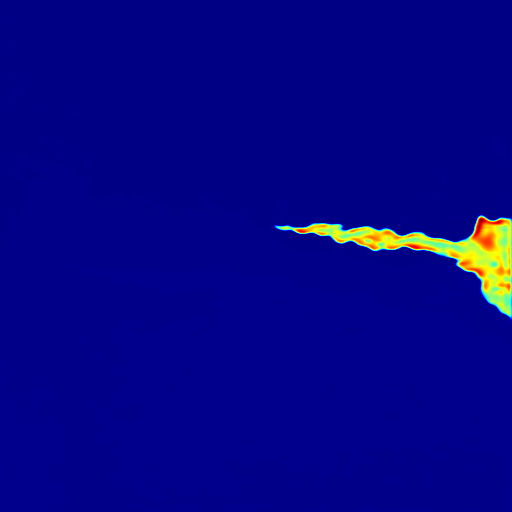
\includegraphics[width=0.6in]{fig7-2-200.png}&
    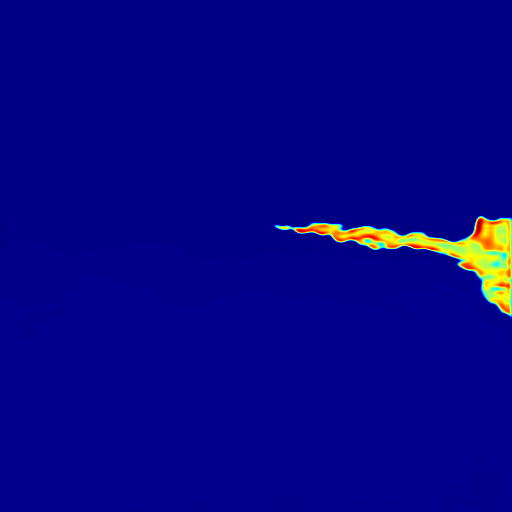
\includegraphics[width=0.6in]{fig7-2-250.png}&
    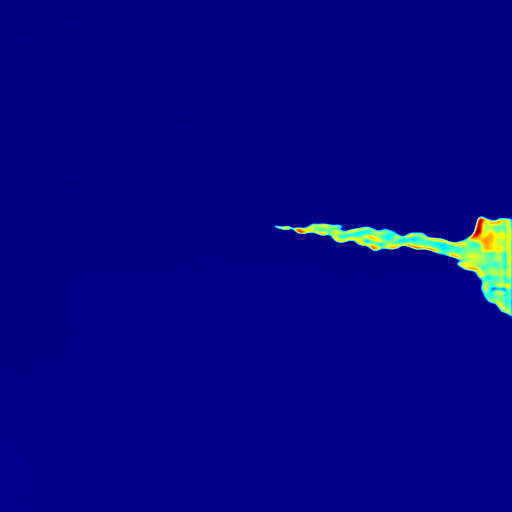
\includegraphics[width=0.6in]{fig7-2-300.png}\\

    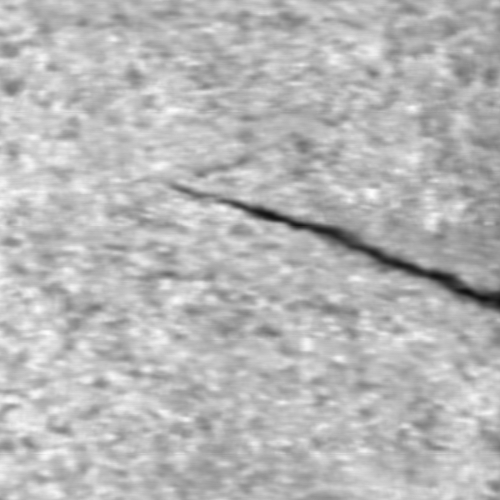
\includegraphics[width=0.6in]{fig7-3.png}&
    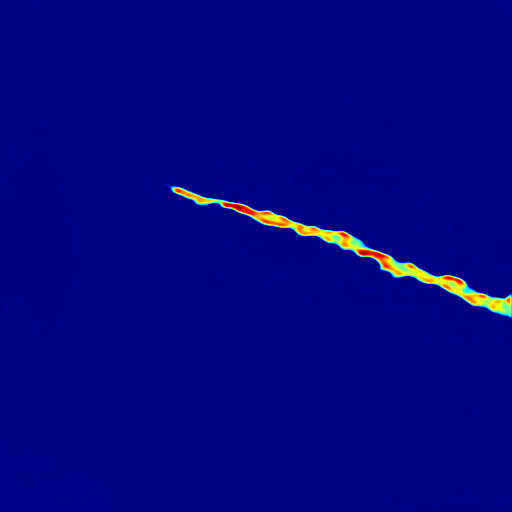
\includegraphics[width=0.6in]{fig7-3-0.png}&
    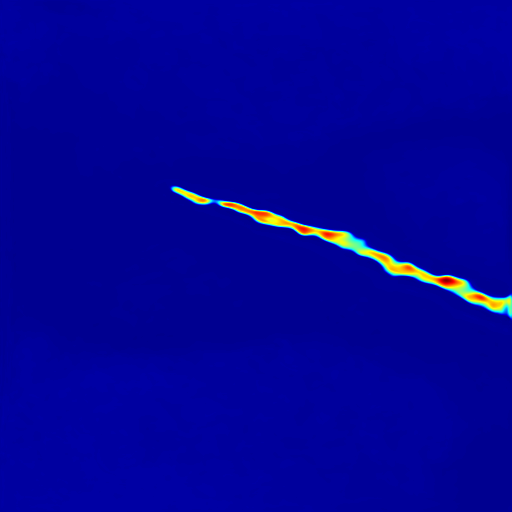
\includegraphics[width=0.6in]{fig7-3-50.png}&
    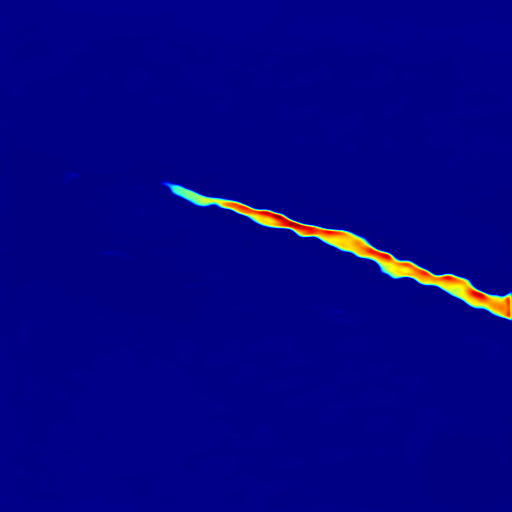
\includegraphics[width=0.6in]{fig7-3-100.png}&
    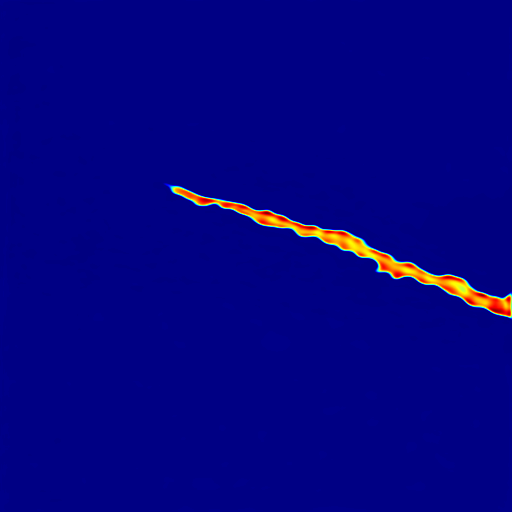
\includegraphics[width=0.6in]{fig7-3-150.png}&
    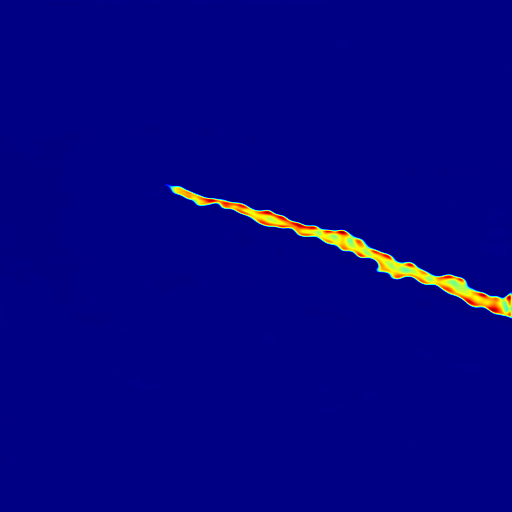
\includegraphics[width=0.6in]{fig7-3-200.png}&
    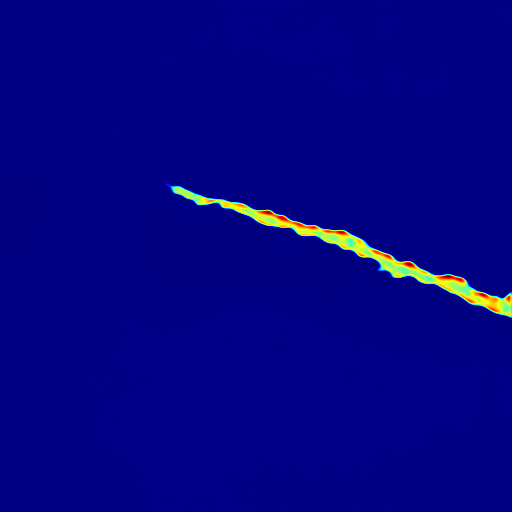
\includegraphics[width=0.6in]{fig7-3-250.png}&
    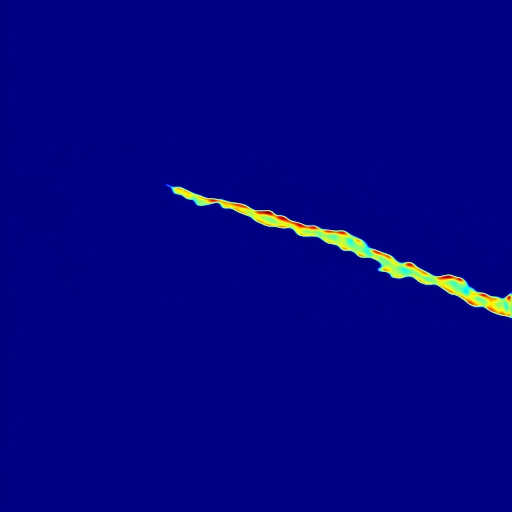
\includegraphics[width=0.6in]{fig7-3-300.png}\\

    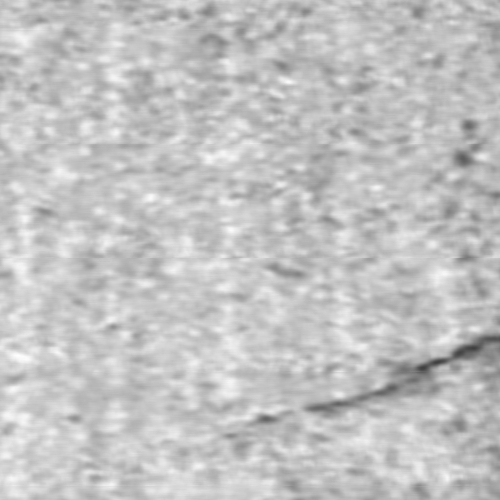
\includegraphics[width=0.6in]{fig7-4.png}&
    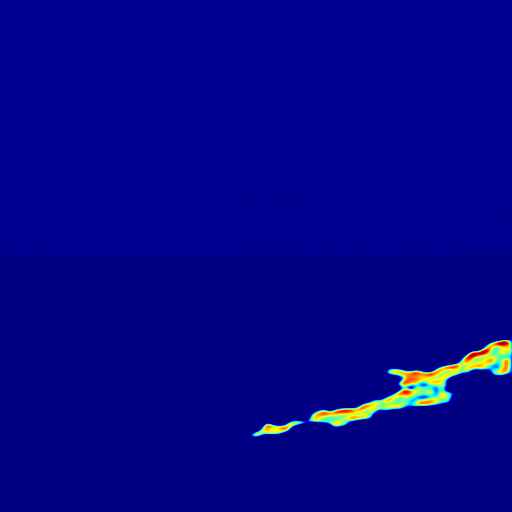
\includegraphics[width=0.6in]{fig7-4-0.png}&
    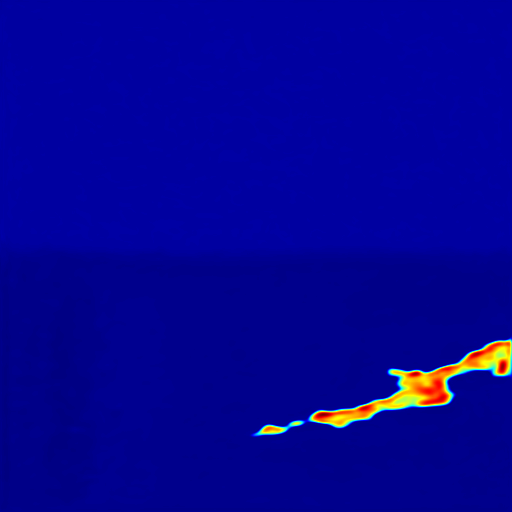
\includegraphics[width=0.6in]{fig7-4-50.png}&
    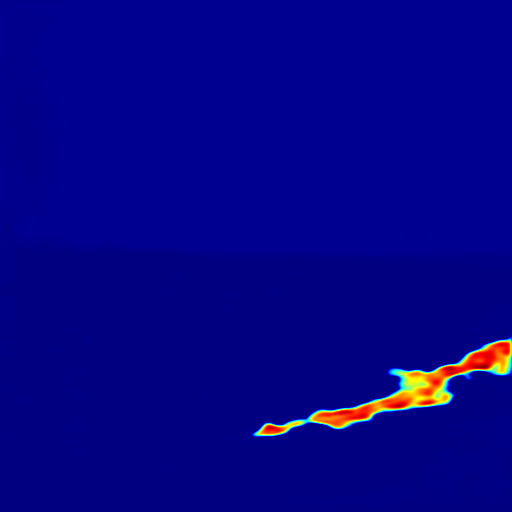
\includegraphics[width=0.6in]{fig7-4-100.png}&
    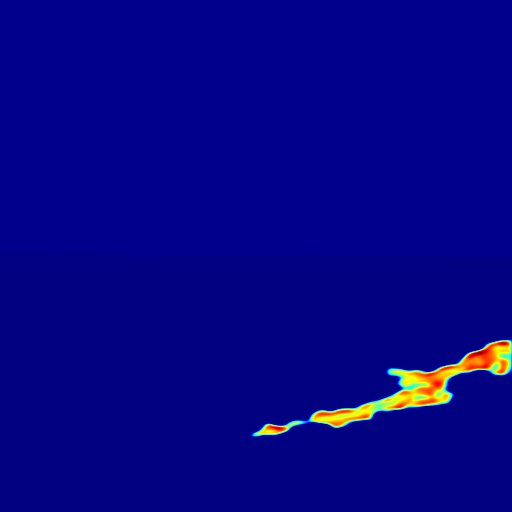
\includegraphics[width=0.6in]{fig7-4-150.png}&
    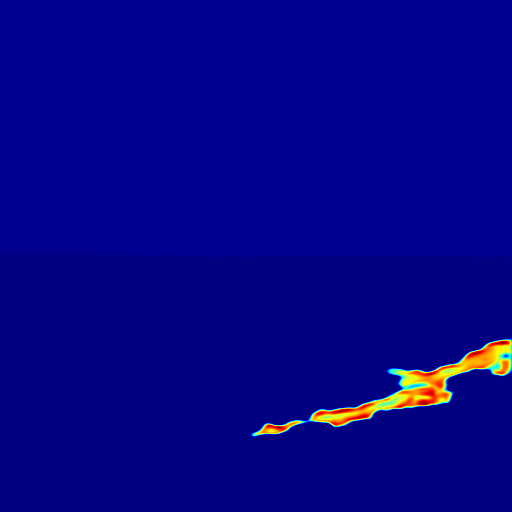
\includegraphics[width=0.6in]{fig7-4-200.png}&
    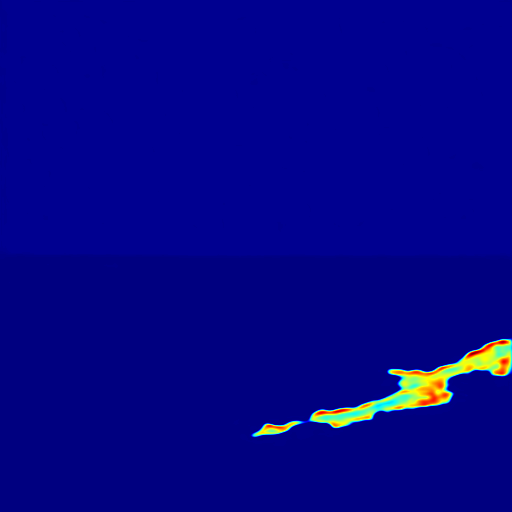
\includegraphics[width=0.6in]{fig7-4-250.png}&
    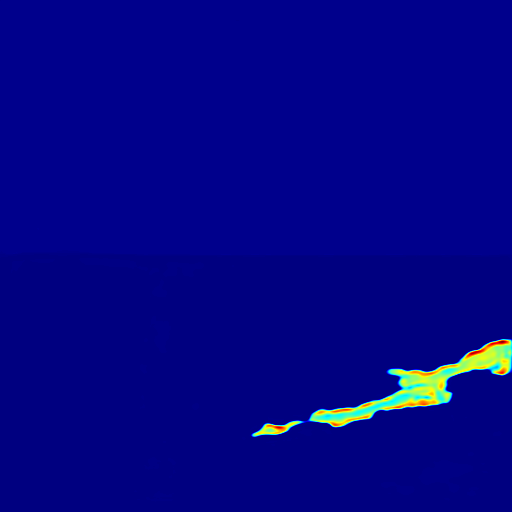
\includegraphics[width=0.6in]{fig7-4-300.png}\\

\centering\rmfamily(a) Img& \centering\rmfamily(b) No& \centering\rmfamily(c) 50& \centering\rmfamily(d) 100& \centering\rmfamily(e) 150& \centering\rmfamily(f) 200& \centering\rmfamily(g) 250& \centering\rmfamily(h) 300\\
\end{tabular}}
	\centering
	\caption{The confidence maps produced without and with data augmentation at different epochs. (a) Image. (b) No. (c) 50. (d) 100. (e) 150. (f) 200. (g) 250. (h) 300. }
	\label{fig:4.2.pix}
\end{figure*}

\begin{figure}
\centering
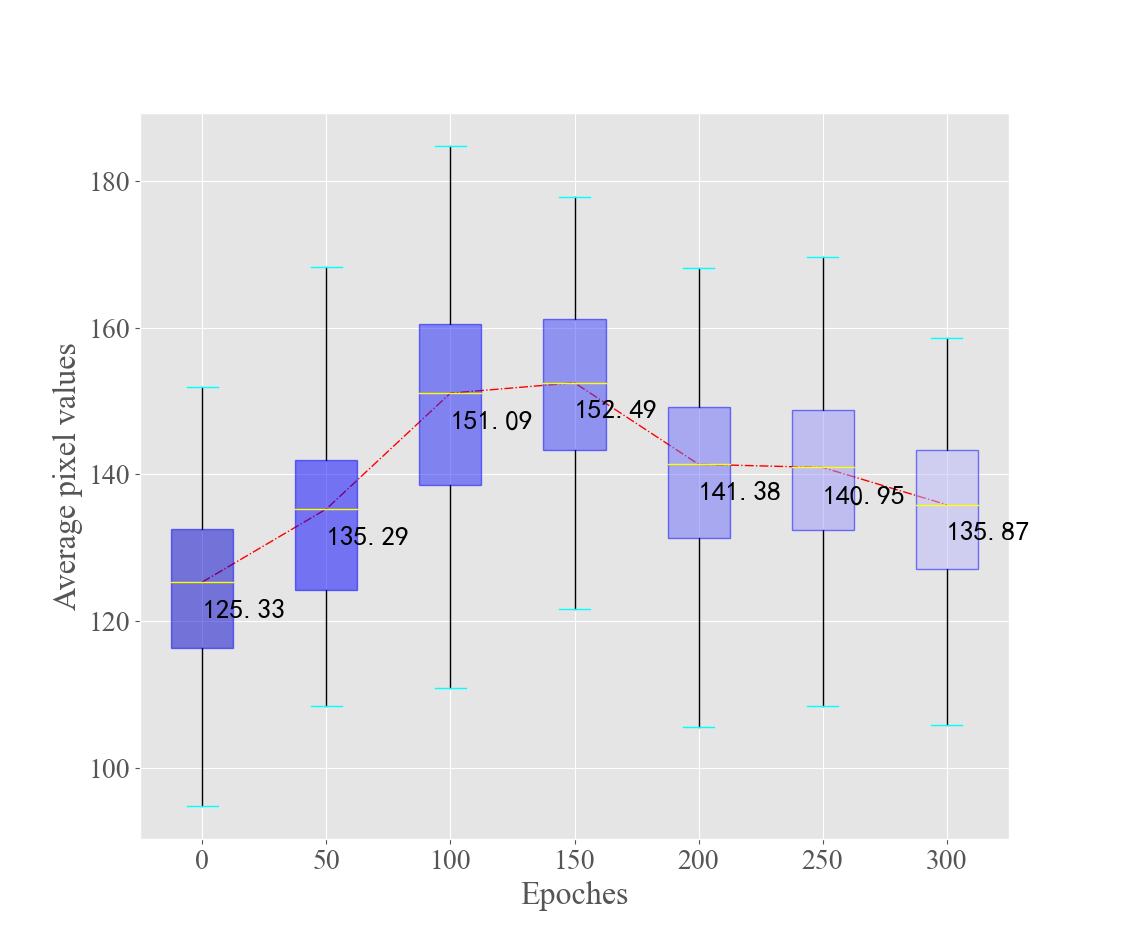
\includegraphics[width=4in]{fig8.png}
\caption{The average value of the confidence map for the defect area within epochs 0-300.}\label{fig:3.pix}
\end{figure}

We conduct experiments to verify the effect of the proposed method on the resulting confidence maps. Fig. \ref{fig:4.2.pix} shows the confidence maps produced with and without the proposed data augmentation. We take the average value of each confidence map for the defect area as the qualitative evaluation standard, as shown in Fig. \ref{fig:3.pix}. 

From Fig. \ref{fig:4.2.pix}, the confidence values of some defect areas are low without data augmentation in column (b), leading to bad segmentation performance. During data augmentation guided by the initial confidence maps in column (b), the model pays significantly more attention to low-confidence regions due to the higher probability of occlusion in high-confidence regions. The confidence values of the defect areas gradually increase and reach their maximum values at epochs 100-150, as shown in Fig. \ref{fig:3.pix}. In particular, the confidence of the regions with low confidence at the start can be significantly improved, as shown in Fig. \ref{fig:4.2.pix}. Because the confidence map exhibits greater differences between the defect areas and the background, it is able to produce better defect segmentation results during data augmentation.

Furthermore, with the guidance confidence maps remaining unchanged, the method first significantly improves the confidence levels of all defect regions and yields their maxima within 100-150 epochs, while the subsequent training process leads to a decrease in the average confidence shown in Fig. \ref{fig:3.pix}.  With a long training time, high-confidence regions are occluded with high probability, which makes it difficult to be noticed by CNN models. The low-confidence region is of greater concern to the model. This results in a transformation of the confidence maps. Training with the original invariant confidence map can lead to overfitting and thus decreased performance. Therefore, we update the confidence map after a period of training to prevent overfitting. According to the above experimental results, the epoch of update cycle $E_{uc}$ in this paper is chosen as 150.

Based on the probability map, the proposed data augmentation method blocks high-probability defect areas and keeps low-probability areas. Therefore, compared to the original image $X$, the defect areas in the augmented image $X_{aug}$ are removed. The retention rate for the defect area $\eta$ represents the ratio of the defect area of $X_{aug}$ to $X$. The range of $\eta$ is originally (0,1). However, when $\eta$ is too high to approach 1, the defect area is not removed. When $\eta$ is too low to approach 0, the defect areas are all deleted. Both of the above are invalid augmentations. To avoid this, we need to limit the range of $\eta$. We construct the experiment which set the range of $\eta$ as (0,1), (0.2,0.8), and (0.4,0.6) separately. Table \ref{tabrange} is the defect segmentation performance under a different range of $\eta$. When the range is (0,1), it causes invalid augmentation. When the range is (0.4, 0.6), $\eta$ is so limited that the randomness is insufficient. When the range is (0.2, 0.8), higher segmentation performance can be obtained. Therefore, we choose the range of $\eta$ to be (0.2, 0.8) based on the experimental results.

\begin{table}[h]
\begin{center}

\caption{The defect segmentation performance on Unet with the different range of $\eta$.}\label{tabrange}%
\begin{tabular}{ccccccccccccc}
\toprule  
The range of $\eta$ &(0.4,0.6)&(0.2,0.8)& (0,1)\\
\midrule
IOU &60.27 &	\textbf{61.97}	 &61.19\\
PA &90.47	 &\textbf{99.51}	 &99.49\\
\botrule

\end{tabular}
\end{center}
\end{table}


\subsection{Comparison with state-of-the-art methods}\label{sec:exp.3}
\label{sec:4.3}
We compare the proposed method with other state-of-the-art methods, which include Cutout \cite{devries2017improved}, HAS \cite{singh2017hide}, GridMask \cite{chen2020gridmask}, and Cutmix \cite{yun2019cutmix}. 
\begin{enumerate}[1)]
\item Cutout \cite{devries2017improved}: Randomly delete image blocks from the input image.
\item HAS \cite{singh2017hide}: Divide the input image into n*n image blocks and delete the image blocks randomly.
\item GridMask \cite{chen2020gridmask}: Build a structured mask and multiply it with the input image.
\item Cutmix \cite{yun2019cutmix}: Perform fusion between two input images at the block level.
\item The proposed method: Occlude low-confidence inputs of input images based on the confidence map obtained by downstream CNN tasks.
\end{enumerate}

We conduct experiments on mainstream segmentation models, including an FCN \cite{long2015fully}, DeepLab \cite{chen2018deeplab:}, and UNet \cite{ronneberger2015u}, which are used by researchers in different industrial surface defect segmentation scenarios.
\begin{enumerate}[1)]
\item \textbf{The FCN} \cite{long2015fully} replaces the fully connected layers in the classic classification network with convolutional layers to obtain a 2-dimensional feature map. It is followed by Softmax activation to obtain the classification information of each pixel. 
\item \textbf{DeepLab} \cite{chen2018deeplab:} adds an atrous spatial pyramid pooling (ASPP) module to the basic ResNet \cite{he2016deep}. ASPP involves atrous convolutions at different sampling rates and global average pooling.
\item \textbf{UNet} \cite{ronneberger2015u} has a U-shaped network structure, which contains an encoder and a decoder. Skip connections are contained between the same stage of the encoder and decoder to ensure that the feature map incorporates more low-level features. UNet is widely used in medical image segmentation and industrial surface defect segmentation.
\end{enumerate}
\begin{table}[h]
\begin{center}
\caption{The segmentation IOU (\%) and PA (\%) achieved on the KSD dataset with the proposed method and other state-of-the-art methods.}\label{tab2}%
\begin{tabular}{p{0.5cm}p{0.8cm}p{0.4cm}p{1cm}p{1cm}p{1cm}p{0.8cm}p{1cm}p{1cm}}
\midrule
\footnotesize $D_{tr}$&\footnotesize $Seg$&\footnotesize $EI$&\footnotesize baseline&\footnotesize Cutmix&\footnotesize Cutout&\footnotesize HAS&\footnotesize GridMask&\footnotesize ours\\
\midrule
 \multirow{6}*{\footnotesize 150}&\multirow{2}*{\footnotesize FCN}& \footnotesize IOU &50.16& 51.59 & 57.02  & 54.10 & 57.20  & \textbf{59.04}\\
 && \footnotesize PA &99.35& 99.35 & 99.43 & 99.41 & 99.44 & \textbf{99.45}\\
\cmidrule{2-9}
 &\multirow{2}*{\footnotesize DeepLab}& \footnotesize IOU &52.98&55.46&57.67&57.65	&57.48& \textbf{58.81}\\
 && \footnotesize PA &99.38&99.41&99.43&99.45&99.44 & \textbf{99.47}\\
\cmidrule{2-9}
 &\multirow{2}*{\footnotesize UNet}& \footnotesize IOU &55.35&58.79&60.90&60.39&59.39 & \textbf{61.97}\\
 && \footnotesize PA &99.45&99.46&99.49&99.48&99.47& \textbf{99.51}\\
\midrule
\multirow{2}*{\footnotesize 80}&\multirow{2}*{\footnotesize UNet}& \footnotesize IOU &54.35&53.15&55.91&56.08&55.70& \textbf{57.63}\\
 && \footnotesize PA &99.40&99.38&99.40&99.42&99.41& \textbf{99.45}\\
\botrule
\end{tabular}
\end{center}
\end{table}

\begin{figure*}
     \setlength{\abovecaptionskip}{0.cm}
     \setlength{\belowcaptionskip}{-0.cm}
	\centering
\scalebox{0.9}{
\begin{tabular}{p{1.2cm}p{1.2cm}p{1.2cm}p{1.2cm}p{1.2cm}p{1.2cm}p{1.2cm}p{1.2cm}}

    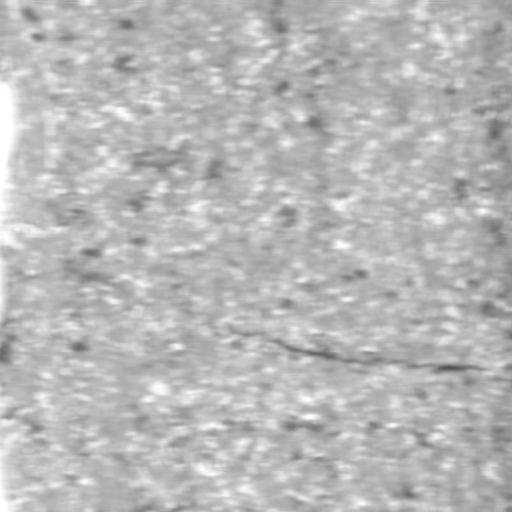
\includegraphics[width=0.6in]{fig9-0-input.png}&
    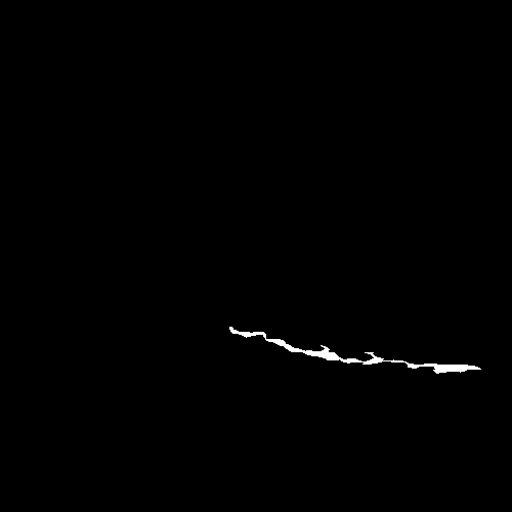
\includegraphics[width=0.6in]{fig9-0-y.png}&
    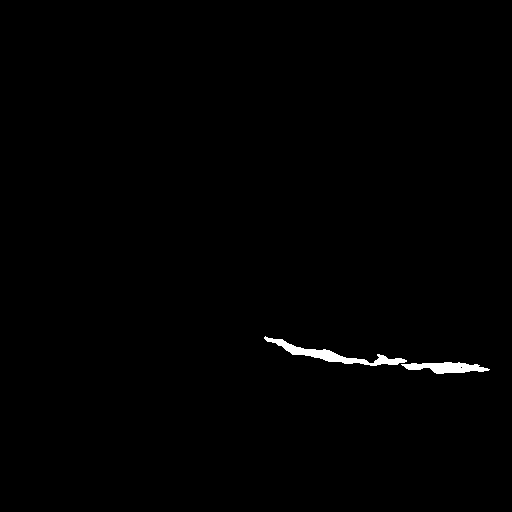
\includegraphics[width=0.6in]{fig9-0-ori.png}&
    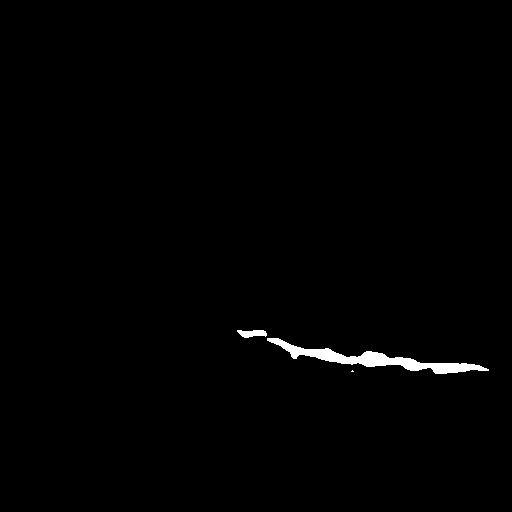
\includegraphics[width=0.6in]{fig9-0-cutmix.png}&
    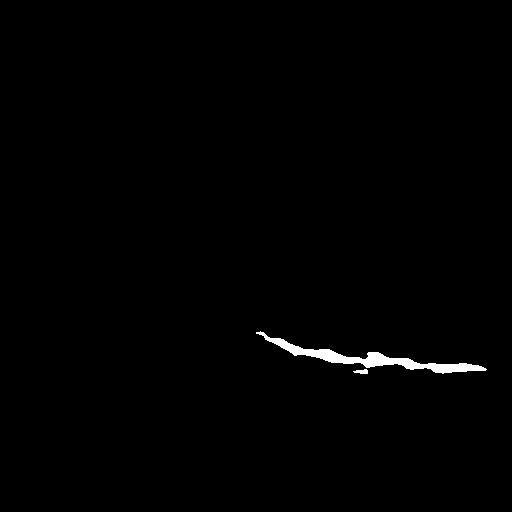
\includegraphics[width=0.6in]{fig9-0-cutout.png}&
    \includegraphics[width=0.6in]{fig9-0-has.png}&
    \includegraphics[width=0.6in]{fig9-0-gridmask.png}&
    \includegraphics[width=0.6in]{fig9-0-ours.png}\\

    \includegraphics[width=0.6in]{fig9-1-input.png}&
    \includegraphics[width=0.6in]{fig9-1-y.png}&
    \includegraphics[width=0.6in]{fig9-1-ori.png}&
    \includegraphics[width=0.6in]{fig9-1-cutmix.png}&
    \includegraphics[width=0.6in]{fig9-1-cutout.png}&
    \includegraphics[width=0.6in]{fig9-1-has.png}&
    \includegraphics[width=0.6in]{fig9-1-gridmask.png}&
    \includegraphics[width=0.6in]{fig9-1-ours.png}\\


    \includegraphics[width=0.6in]{fig9-2-input.png}&
    \includegraphics[width=0.6in]{fig9-2-y.png}&
    \includegraphics[width=0.6in]{fig9-2-ori.png}&
    \includegraphics[width=0.6in]{fig9-2-cutmix.png}&
    \includegraphics[width=0.6in]{fig9-2-cutout.png}&
    \includegraphics[width=0.6in]{fig9-2-has.png}&
    \includegraphics[width=0.6in]{fig9-2-gridmask.png}&
    \includegraphics[width=0.6in]{fig9-2-ours.png}\\

\centering\footnotesize(a)Img& \centering\footnotesize(b)Label& \centering\footnotesize(c)Baseline& \centering\footnotesize(d)Cutmix& \centering\footnotesize(e)Cutout& \centering\footnotesize(f)HAS& \centering\footnotesize(g)GridMask & \centering\footnotesize(h)Ours\\
\end{tabular}}
	\centering
	\caption{Defect segmentation results obtained without data augmentation and with various state-of-the-art data augmentation methods. (a) Image. (b) Label. (c) Baseline. (d) Cutmix. (e) Cutout. (f) HAS. (g) GridMask. (h) Ours.  }
	\label{fig:4.3.KSD}
\end{figure*}


The comparison between the proposed data augmentation method and other state-of-the-art methods is shown in Table \ref{tab2}. Our method has significantly better accuracy than the baseline without data augmentation. 
Compared with other state-of-the-art methods, the proposed method also obtains higher segmentation accuracy.
Moreover, the proposed data augmentation method can effectively improve the accuracy of defect segmentation when using different mainstream defect segmentation networks, such as UNet \cite{ronneberger2015u}, DeepLab \cite{chen2018deeplab:}, and an FCN \cite{long2015fully}, which demonstrates the generality of our method for mainstream defect segmentation methods.

Fig.\ref{fig:4.3.KSD} shows the segmentation results obtained by different data augmentation methods on UNet. For defects with normal intensities shown in the first line, the segmentation models with and without data augmentation can achieve accurate segmentation. However, for defects with weak intensities in the last two lines, the baseline cannot perform effective segmentation. All kinds of data augmentation methods can effectively improve the segmentation results of weak defects. However, other data augmentation methods, such as HAS\cite{singh2017hide} and GridMask \cite{chen2020gridmask}, cannot fully and accurately identify defects of weak features. Compared to other data augmentation methods, the proposed method yields more obvious improvements for weak defects and thus obtains more accurate segmentation results.

\begin{figure}
\centering
\includegraphics[width=4in]{fig10.png}
\caption{The average value of the confidence maps for different methods.}\label{fig:3.avemethod}
\end{figure}

\begin{figure*}
     \setlength{\abovecaptionskip}{0.cm}
     \setlength{\belowcaptionskip}{-0.cm}
	\centering
\scalebox{0.9}{
\begin{tabular}{p{1.5cm}p{1.5cm}p{1.5cm}p{1.5cm}p{1.5cm}p{1.5cm}p{1.5cm}}


    \includegraphics[width=0.65in]{fig11-0-input.png}& 
    \includegraphics[width=0.65in]{fig11-0-ori.png}& 
    \includegraphics[width=0.65in]{fig11-0-cutmix.png}& 
    \includegraphics[width=0.65in]{fig11-0-cutout.png}& 
    \includegraphics[width=0.65in]{fig11-0-has.png}& 
    \includegraphics[width=0.65in]{fig11-0-gridmask.png}& 
    \includegraphics[width=0.65in]{fig11-0-ours.png} \\

    \includegraphics[width=0.65in]{fig11-1-input.png}& 
    \includegraphics[width=0.65in]{fig11-1-ori.png}& 
    \includegraphics[width=0.65in]{fig11-1-cutmix.png}& 
    \includegraphics[width=0.65in]{fig11-1-cutout.png}& 
    \includegraphics[width=0.65in]{fig11-1-has.png}& 
    \includegraphics[width=0.65in]{fig11-1-gridmask.png}& 
    \includegraphics[width=0.65in]{fig11-1-ours.png} \\

    \includegraphics[width=0.65in]{fig11-2-input.png}& 
    \includegraphics[width=0.65in]{fig11-2-ori.png}& 
    \includegraphics[width=0.65in]{fig11-2-cutmix.png}& 
    \includegraphics[width=0.65in]{fig11-2-cutout.png}& 
    \includegraphics[width=0.65in]{fig11-2-has.png}& 
    \includegraphics[width=0.65in]{fig11-2-gridmask.png}& 
    \includegraphics[width=0.65in]{fig11-2-ours.png} \\

\centering\footnotesize(a)Img& \centering\footnotesize(b)Baseline& \centering\footnotesize(c)Cutmix& \centering\footnotesize(d)Cutout& \centering\footnotesize(e)HAS& \centering\footnotesize(f)GridMask & \centering\footnotesize(g)Ours\\
\end{tabular}}
	\centering
	\caption{Confidence maps for different methods. (a) Image. (b) Baseline. (c) Cutmix. (d) Cutout. (e) HAS. (f) GridMask. (g) Ours.  }
	\label{fig:4.3.KSD-cm}
\end{figure*}

We also analyze the confidence maps for different methods. We use the average pixel of the confidence map for the defect area as the quantitative evaluation. As shown in Fig. \ref{fig:3.avemethod}, compared with other methods, the average value obtained by the proposed method is higher, which indicates that our method can obtain a more significant confidence map. Fig. \ref{fig:4.3.KSD-cm} shows the confidence map for different methods. Specifically,  although different methods can obtain similar detection results in the first line, our method can obtain a better confidence map for the defects with normal intensities, which shows that the segmentation model constructed by the proposed method has higher confidence for the defect area.  Although Cutout \cite{devries2017improved} can also obtain relatively good detection results for weak feature defects in the last two lines, the proposed method can obtain more significant confidence maps than Cutout \cite{devries2017improved}.

The proposed data augmentation method can perform occlusion adjustment on the input image of the training set based on the probability map. Although the other methods Cutout \cite{devries2017improved}, HAS\cite{singh2017hide} and GridMask \cite{chen2020gridmask} also occlude the input image, the occluded region is random, which causes invalid augmentation. The proposed method essentially increases the exposure of low-confidence regions in the model so that the model pays more attention to low-confidence regions. Moreover, the purpose of data augmentation is to improve the performance of subsequent defect segmentation. Therefore, starting from the requirements of the defect segmentation model, the proposed data augmentation is to improve the degree of attention to low-confidence regions by the downstream CNN. Therefore, the proposed method can obtain more salient feature maps, including the hard-to-detect regions and thus obtain more accurate segmentation results. Moreover, difficult-to-detect regions often represent some weak feature defects, such as weak contrast defects. Therefore, the proposed method can significantly improve the detection ability of defects with weak features.


In order to verify data augmentation in the case of different data volume levels, we reduce the training set $D_{tr}$ from 150 to 80. As shown in Table \ref{tab2}, compared with other methods, the proposed method can further significantly increase the defect segmentation accuracy over the baseline with the smaller training set. This shows the effectiveness of our method under different data volumes.

\subsection{An application of the proposed method}\label{sec:exp.app}

\begin{figure}
\centering
\includegraphics[width=3in]{fig12.jpg}
\caption{Diagram of an optoelectronic chip and a waveguide. Waveguide defects and bubble defects appear on the wafer.}\label{fig:3.8}
\end{figure}

The proposed method is applied to an actual optoelectronic chip production line. An optoelectronic chip is an important component of optical communication equipment. As shown in Fig. \ref{fig:3.8}, a large number of waveguide lines are arranged on the optoelectronic chips of a wafer for the propagation of optical information. During the manufacturing process, due to the small sizes and dense arrangement of the optical waveguides, waveguide defects (WDs), such as breakages or crossovers, may occur, affecting the efficiency and accuracy of the optical wave transmission process. Moreover, the packaging of the optoelectronic chips may cause bubble defects (BDs). We construct an optical chip defect dataset named OCDD, which contains a total of 317 BD images and 224 WD images. We randomly divide the training set and test set at a ratio of 2:1. 

\begin{table}[h]
\begin{center}

\caption{The defect segmentation performance of the proposed methods and other state-of-the-art methods on an optoelectronic chip.}\label{tab3}%
\begin{tabular}{ccccccccccccc}
\toprule  

 Method & $EI$ & baseline & Cutout & HAS & GirdMask & Cutmix & ours\\
\midrule
\multirow{2}*{WD}&IOU&51.05&56.86&56.32&52.63&55.47&\textbf{58.38}\\
&PA&99.41&99.46&99.46&99.43&99.44&\textbf{99.48}\\
\midrule
\multirow{2}*{BD}&IOU&69.89&66.17&69.10&66.23&69.30&\textbf{69.90}\\
&PA&98.82&99.30&\textbf{99.37}&99.30&99.17&99.28\\
\midrule
\multirow{2}*{Total}&IOU&61.75&62.13&63.95&60.96&63.87&\textbf{64.91}\\
&PA&99.08&99.32&\textbf{99.40}&99.35&99.29&99.37\\
\botrule

\end{tabular}
\end{center}
\end{table}

\begin{figure*}
     \setlength{\abovecaptionskip}{0.cm}
     \setlength{\belowcaptionskip}{-0.cm}
	\centering
\scalebox{0.9}{
\begin{tabular}{p{1.3cm}p{1.3cm}p{1.3cm}p{1.3cm}p{1.3cm}p{1.3cm}p{1.3cm}p{1.3cm}}

    \includegraphics[width=0.65in]{fig13-bodao36inputs.png}&
    \includegraphics[width=0.65in]{fig13-bodao36y.png}&
    \includegraphics[width=0.65in]{fig13-bodao36baseline.png}&
    \includegraphics[width=0.65in]{fig13-bodao36cutout.png}&
    \includegraphics[width=0.65in]{fig13-bodao36has.png}&
    \includegraphics[width=0.65in]{fig13-bodao36gridmask.png}&
    \includegraphics[width=0.65in]{fig13-bodao36cutmix.png}&
    \includegraphics[width=0.65in]{fig13-bodao36ours.png}\\
    \includegraphics[width=0.65in]{fig13-bodao55inputs.png}&
    \includegraphics[width=0.65in]{fig13-bodao55y.png}&
    \includegraphics[width=0.65in]{fig13-bodao55baseline.png}&
    \includegraphics[width=0.65in]{fig13-bodao55cutout.png}&
    \includegraphics[width=0.65in]{fig13-bodao55has.png}&
    \includegraphics[width=0.65in]{fig13-bodao55gridmask.png}&
    \includegraphics[width=0.65in]{fig13-bodao55cutmix.png}&
    \includegraphics[width=0.65in]{fig13-bodao55ours.png}\\
    \includegraphics[width=0.65in]{fig13-qipao44inputs.png}&
    \includegraphics[width=0.65in]{fig13-qipao44y.png}&
    \includegraphics[width=0.65in]{fig13-qipao44baseline.png}&
    \includegraphics[width=0.65in]{fig13-qipao44cutout.png}&
    \includegraphics[width=0.65in]{fig13-qipao44has.png}&
    \includegraphics[width=0.65in]{fig13-qipao44gridmask.png}&
    \includegraphics[width=0.65in]{fig13-qipao44cutmix.png}&
    \includegraphics[width=0.65in]{fig13-qipao44ours.png}\\
    \includegraphics[width=0.65in]{fig13-qipao28inputs.png}&
    \includegraphics[width=0.65in]{fig13-qipao28y.png}&
    \includegraphics[width=0.65in]{fig13-qipao28baseline.png}&
    \includegraphics[width=0.65in]{fig13-qipao28cutout.png}&
    \includegraphics[width=0.65in]{fig13-qipao28has.png}&
    \includegraphics[width=0.65in]{fig13-qipao28gridmask.png}&
    \includegraphics[width=0.65in]{fig13-qipao28cutmix.png}&
    \includegraphics[width=0.65in]{fig13-qipao28ours.png}\\

\centering\rmfamily\scriptsize (a)Img& \centering\rmfamily\scriptsize(b)Label& \centering\rmfamily\scriptsize(c)Baseline& \centering\rmfamily\scriptsize(d)Cutout& \centering\rmfamily\scriptsize(e)HAS& \centering\rmfamily\scriptsize(f)Grdmask& \centering\rmfamily\scriptsize(g)CutMix& \centering\rmfamily\scriptsize(h)Ours\\
\end{tabular}}
	\centering
	\caption{Defect segmentation results of the optoelectronic chip obtained without data augmentation and with our data augmentation method. (a) Image. (b) Label. (c) Baseline. (d) Cutout.(e)HAS.(f) GridMask. (g) CutMix. (h) Ours.}
	\label{fig:4.light222}
\end{figure*}

We construct comparative experiments for OCDD with the proposed method and other state-of-the-art methods. 
Based on the results in Section \ref{sec:4.3}, we employ UNet \cite{ronneberger2015u} and the proposed data augmentation method to construct a segmentation model. The baseline is UNet \cite{ronneberger2015u} without any data augmentation.
As shown in Table \ref{tab3}, the proposed data augmentation approach significantly improves the accuracy of defect segmentation and achieves higher accuracy than the other methods. 
Furthermore, as shown in Fig. \ref{fig:4.light222}, the proposed data augmentation method can effectively detect the WDs with weak features, such as those with similar background colors (green boxes) and small areas (yellow boxes), which cannot be effectively detected by the baseline without data augmentation and other methods. The proposed data augmentation method can also detect BDs (red boxes) more completely than the baseline, which is very important for judging the severity of defects. Since the optoelectronic chip detection accuracy is limited by the defects with weak features and a small area, which are of greater concern to the engineers, the proposed method can be effectively applied in optoelectronic chip defect detection scenarios.

\subsection{Discussion}\label{sec:exp.app}
The information density of different image features is different. For example, defect features that are frequent and easy to detect tend to have a lower density, whereas rare and difficult-to-detect defect features tend to have higher density. In this paper, high-confidence defect regions have lower information density, whereas low-confidence defect regions have higher information density for CNN.
During the CNN training process, a large amount of redundant feature information, such as similar defect features, occupies the model's attention and causes model degradation \cite{lin2017focal}; this is called the easy sample overwhelming problem. 

The essence of data augmentation is the resampling and combination of existing feature information. Therefore, more attention should be paid to feature information with higher density during resampling for data augmentation. 
As mentioned above, mainstream data augmentation methods, such as GANs and Cutout \cite{devries2017improved}, are random and do not focus on defective samples with higher information density. Moreover, the GAN training process itself has a mode collapse problem, which tends to generate repeated samples with low density, contrary to the original intention of data augmentation.
The main strategy of the proposed data augmentation approach is to remove low-density areas to increase the attention of the CNN model to high-density regions. This technique is essentially based on the idea of hard sample mining, which is performed at the pixel level instead of at the image level.

\section{Conclusion}\label{sec:con}
In this paper, we propose a simple plug-and-play defect image augmentation method based on CNN requirements, which can be directly applied to existing defect segmentation methods. The proposed method utilizes confidence maps to remove the high-confidence regions of an image to suppress the attention to easy-to-detect areas and increase the attention to difficult-to-detect areas. We construct adequate quantitative and qualitative experiments on metal surfaces and optical chips to compare our method with state-of-the-art data augmentation approaches. 
The experimental results show that the proposed method can effectively achieve improved segmentation performance, especially for defects with weak features, and is suitable for different mainstream defect segmentation models.

In the future, some technical issues can still be further improved, and the proposed method can be extended. 1) This paper is based on the confidence map obtained from the segmentation model to guide data augmentation. In the follow-up, we can further design specific performance indicators to guide data augmentation according to other needs of the industrial site. 2) We can further apply the idea of performing data augmentation based on CNN requirements to various industrial vision tasks, such as defect classification and defect object detection. 

\section*{Acknowledgments}

This work was supported in part by the National Key R\&D Program of China under Grant 2018YFB1700500 and the Key Research and Development Program of HubeiChina (2020BAB106).

\begin{thebibliography}{10}

\bibitem{hu2020an}
Chuanfei {Hu} and Yongxiong {Wang}.
\newblock An efficient convolutional neural network model based on object-level
  attention mechanism for casting defect detection on radiography images.
\newblock {\em IEEE Transactions on Industrial Electronics},
  67(12):10922--10930, 2020.

\bibitem{dong2020pga}
Hongwen {Dong}, Kechen {Song}, Yu~{He}, Jing {Xu}, Yunhui {Yan}, and Qinggang
  {Meng}.
\newblock Pga-net: Pyramid feature fusion and global context attention network
  for automated surface defect detection.
\newblock {\em IEEE Transactions on Industrial Informatics}, 16(12):7448--7458,2020.

\bibitem{su2021deep}
Binyi {Su}, Hai yong {Chen}, Peng {Chen}, Gui-Bin {Bian}, kun {Liu}, and
  Weipeng {Liu}.
\newblock Deep learning-based solar-cell manufacturing defect detection with
  complementary attention network.
\newblock {\em IEEE Transactions on Industrial Informatics}, 17(6):4084--4095,
  2021.

\bibitem{kim2021wafer}
Yusung Kim, Donghee Cho, and Jee-Hyong Lee.
\newblock Wafer defect pattern classification with detecting
  out-of-distribution.
\newblock {\em Microelectronics Reliability}, 122:114157, 2021.

\bibitem{cheng2021machine}
Ken Chau-Cheung Cheng, Leon Li-Yang Chen, Ji-Wei Li, Katherine Shu-Min Li, Nova
  Cheng-Yen Tsai, Sying-Jyan Wang, Andrew Yi-Ann Huang, Leon Chou, Chen-Shiun
  Lee, Jwu~E Chen, et~al.
\newblock Machine learning-based detection method for wafer test induced
  defects.
\newblock {\em IEEE Transactions on Semiconductor Manufacturing},
  34(2):161--167, 2021.

\bibitem{chen2020gridmask}
Pengguang Chen, Shu Liu, Hengshuang Zhao, and Jiaya Jia.
\newblock Gridmask data augmentation.
\newblock {\em arXiv preprint arXiv:2001.04086}, 2020.

\bibitem{krizhevsky2012imagenet}
Alex Krizhevsky, Ilya Sutskever, and Geoffrey~E Hinton.
\newblock Imagenet classification with deep convolutional neural networks.
\newblock {\em Advances in neural information processing systems}, 25, 2012.

\bibitem{goodfellow2014generative}
Ian~J Goodfellow, Jean Pouget-Abadie, Mehdi Mirza, Bing Xu, David Warde-Farley,
  Sherjil Ozair, Aaron Courville, and Yoshua Bengio.
\newblock Generative adversarial networks.
\newblock {\em arXiv preprint arXiv:1406.2661}, 2014.

\bibitem{kingma2013auto}
Diederik~P Kingma and Max Welling.
\newblock Auto-encoding variational bayes.
\newblock {\em arXiv preprint arXiv:1312.6114}, 2013.

\bibitem{isola2017image}
Phillip {Isola}, Jun-Yan {Zhu}, Tinghui {Zhou}, and Alexei~A. {Efros}.
\newblock Image-to-image translation with conditional adversarial networks.
\newblock In {\em 2017 IEEE Conference on Computer Vision and Pattern
  Recognition (CVPR)}, pages 5967--5976, 2017.

\bibitem{choi2018stargan}
Yunjey {Choi}, Minje {Choi}, Munyoung {Kim}, Jung-Woo {Ha}, Sunghun {Kim}, and
  Jaegul {Choo}.
\newblock Stargan: Unified generative adversarial networks for multi-domain
  image-to-image translation.
\newblock In {\em 2018 IEEE/CVF Conference on Computer Vision and Pattern
  Recognition}, pages 8789--8797, 2018.

\bibitem{zheng2017unlabeled}
Zhedong Zheng, Liang Zheng, and Yi~Yang.
\newblock Unlabeled samples generated by gan improve the person
  re-identification baseline in vitro.
\newblock In {\em Proceedings of the IEEE international conference on computer
  vision}, pages 3754--3762, 2017.

\bibitem{wang2017adversarial}
Xinlong Wang, Zhipeng Man, Mingyu You, and Chunhua Shen.
\newblock Adversarial generation of training examples: applications to moving
  vehicle license plate recognition.
\newblock {\em arXiv preprint arXiv:1707.03124}, 2017.

\bibitem{fan2021learning}
Rui Fan, Hengli Wang, Peide Cai, Jin Wu, Junaid Bocus, Lei Qiao, and Ming Liu.
\newblock Learning collision-free space detection from stereo images:
  Homography matrix brings better data augmentation.
\newblock {\em IEEE/ASME Transactions on Mechatronics}, 2021.

\bibitem{devries2017improved}
Terrance DeVries and Graham~W Taylor.
\newblock Improved regularization of convolutional neural networks with cutout.
\newblock {\em arXiv preprint arXiv:1708.04552}, 2017.

\bibitem{muller2021trivialaugment}
Samuel~G M{\"u}ller and Frank Hutter.
\newblock Trivialaugment: Tuning-free yet state-of-the-art data augmentation.
\newblock In {\em Proceedings of the IEEE/CVF International Conference on
  Computer Vision}, pages 774--782, 2021.

\bibitem{singh2017hide}
Krishna~Kumar Singh and Yong~Jae Lee.
\newblock Hide-and-seek: Forcing a network to be meticulous for
  weakly-supervised object and action localization.
\newblock In {\em 2017 IEEE international conference on computer vision
  (ICCV)}, pages 3544--3553. IEEE, 2017.

\bibitem{zhang2017mixup}
Hongyi Zhang, Moustapha Cisse, Yann~N Dauphin, and David Lopez-Paz.
\newblock mixup: Beyond empirical risk minimization.
\newblock {\em arXiv preprint arXiv:1710.09412}, 2017.

\bibitem{yun2019cutmix}
Sangdoo Yun, Dongyoon Han, Seong~Joon Oh, Sanghyuk Chun, Junsuk Choe, and
  Youngjoon Yoo.
\newblock Cutmix: Regularization strategy to train strong classifiers with
  localizable features.
\newblock In {\em Proceedings of the IEEE/CVF international conference on
  computer vision}, pages 6023--6032, 2019.

\bibitem{hendrycks2019augmix}
Dan Hendrycks, Norman Mu, Ekin~D Cubuk, Barret Zoph, Justin Gilmer, and Balaji
  Lakshminarayanan.
\newblock Augmix: A simple data processing method to improve robustness and
  uncertainty.
\newblock {\em arXiv preprint arXiv:1912.02781}, 2019.

\bibitem{chen2021transmix}
Jie-Neng Chen, Shuyang Sun, Ju~He, Philip Torr, Alan Yuille, and Song Bai.
\newblock Transmix: Attend to mix for vision transformers.
\newblock {\em arXiv preprint arXiv:2111.09833}, 2021.

\bibitem{ghiasi2021simple}
Golnaz Ghiasi, Yin Cui, Aravind Srinivas, Rui Qian, Tsung-Yi Lin, Ekin~D Cubuk,
  Quoc~V Le, and Barret Zoph.
\newblock Simple copy-paste is a strong data augmentation method for instance
  segmentation.
\newblock In {\em Proceedings of the IEEE/CVF Conference on Computer Vision and
  Pattern Recognition}, pages 2918--2928, 2021.


\bibitem{zheng2019joint}
Zhedong Zheng, Xiaodong Yang, Zhiding Yu, Liang Zheng, Yi~Yang, and Jan Kautz.
\newblock Joint discriminative and generative learning for person
  re-identification.
\newblock In {\em proceedings of the IEEE/CVF conference on computer vision and
  pattern recognition}, pages 2138--2147, 2019.

\bibitem{lin2020gan}
Che-Tsung Lin, Sheng-Wei Huang, Yen-Yi Wu, and Shang-Hong Lai.
\newblock Gan-based day-to-night image style transfer for nighttime vehicle
  detection.
\newblock {\em IEEE Transactions on Intelligent Transportation Systems},
  22(2):951--963, 2020.

\bibitem{uricar2021let}
Michal Uricar, Ganesh Sistu, Hazem Rashed, Antonin Vobecky, Varun~Ravi Kumar,
  Pavel Krizek, Fabian Burger, and Senthil Yogamani.
\newblock Let's get dirty: Gan based data augmentation for camera lens soiling
  detection in autonomous driving.
\newblock In {\em Proceedings of the IEEE/CVF Winter Conference on Applications
  of Computer Vision}, pages 766--775, 2021.

\bibitem{choi2019self}
Jaehoon Choi, Taekyung Kim, and Changick Kim.
\newblock Self-ensembling with gan-based data augmentation for domain
  adaptation in semantic segmentation.
\newblock In {\em Proceedings of the IEEE/CVF International Conference on
  Computer Vision}, pages 6830--6840, 2019.

\bibitem{zhang2020robust}
Linjiang Zhang, Peng Wang, Hui Li, Zhen Li, Chunhua Shen, and Yanning Zhang.
\newblock A robust attentional framework for license plate recognition in the
  wild.
\newblock {\em IEEE Transactions on Intelligent Transportation Systems},
  22(11):6967--6976, 2020.

\bibitem{zhu2017unpaired}
Jun-Yan Zhu, Taesung Park, Phillip Isola, and Alexei~A Efros.
\newblock Unpaired image-to-image translation using cycle-consistent
  adversarial networks.
\newblock In {\em Proceedings of the IEEE international conference on computer
  vision}, pages 2223--2232, 2017.

\bibitem{bissoto2021gan}
Alceu Bissoto, Eduardo Valle, and Sandra Avila.
\newblock Gan-based data augmentation and anonymization for skin-lesion
  analysis: A critical review.
\newblock In {\em Proceedings of the IEEE/CVF Conference on Computer Vision and
  Pattern Recognition}, pages 1847--1856, 2021.

\bibitem{naghizadeh2021semantic}
Alireza Naghizadeh, Hongye Xu, Mohab Mohamed, Dimitris~N Metaxas, and Dongfang
  Liu.
\newblock Semantic aware data augmentation for cell nuclei microscopical images
  with artificial neural networks.
\newblock In {\em Proceedings of the IEEE/CVF International Conference on
  Computer Vision}, pages 3952--3961, 2021.

\bibitem{luo2021fa}
Mandi Luo, Jie Cao, Xin Ma, Xiaoyu Zhang, and Ran He.
\newblock Fa-gan: face augmentation gan for deformation-invariant face
  recognition.
\newblock {\em IEEE Transactions on Information Forensics and Security},
  16:2341--2355, 2021.

\bibitem{hsu2021multiple}
Chia-Yu Hsu and Wei-Chen Liu.
\newblock Multiple time-series convolutional neural network for fault detection
  and diagnosis and empirical study in semiconductor manufacturing.
\newblock {\em Journal of Intelligent Manufacturing}, 32(3):823--836, 2021.

\bibitem{schlosser2022improving}
Tobias Schlosser, Michael Friedrich, Frederik Beuth, and Danny Kowerko.
\newblock Improving automated visual fault inspection for semiconductor
  manufacturing using a hybrid multistage system of deep neural networks.
\newblock {\em Journal of Intelligent Manufacturing}, 33(4):1099--1123, 2022.

\bibitem{sassi2019smart}
Paolo Sassi, Paolo Tripicchio, and Carlo~Alberto Avizzano.
\newblock A smart monitoring system for automatic welding defect detection.
\newblock {\em IEEE Transactions on Industrial Electronics}, 66(12):9641--9650,
  2019.

\bibitem{pan2021artificial}
Ligong Pan, Rodion Rogulin, and Sergey Kondrashev.
\newblock Artificial neural network for defect detection in ct images of wood.
\newblock {\em Computers and Electronics in Agriculture}, 187:106312, 2021.

\bibitem{jain2020synthetic}
Saksham Jain, Gautam Seth, Arpit Paruthi, Umang Soni, and Girish Kumar.
\newblock Synthetic data augmentation for surface defect detection and
  classification using deep learning.
\newblock {\em Journal of Intelligent Manufacturing}, pages 1--14, 2020.

\bibitem{xuan2018multiview}
Qi~Xuan, Zhuangzhi Chen, Yi~Liu, Huimin Huang, Guanjun Bao, and Dan Zhang.
\newblock Multiview generative adversarial network and its application in pearl
  classification.
\newblock {\em IEEE Transactions on Industrial Electronics}, 66(10):8244--8252,
  2018.

\bibitem{niu2020defect}
Shuanlong Niu, Bin Li, Xinggang Wang, and Hui Lin.
\newblock Defect image sample generation with gan for improving defect
  recognition.
\newblock {\em IEEE Transactions on Automation Science and Engineering},
  17(3):1611--1622, 2020.

\bibitem{le2020learning}
Xinyi Le, Junhui Mei, Haodong Zhang, Boyu Zhou, and Juntong Xi.
\newblock A learning-based approach for surface defect detection using small
  image datasets.
\newblock {\em Neurocomputing}, 408:112--120, 2020.

\bibitem{yang2021mask2defect}
Benyi Yang, Zhenyu Liu, Guifang Duan, and Jianrong Tan.
\newblock Mask2defect: A prior knowledge based data augmentation method for
  metal surface defect inspection.
\newblock {\em IEEE Transactions on Industrial Informatics}, 2021.

\bibitem{yun2020automated}
Jong~Pil Yun, Woosang~Crino Shin, Gyogwon Koo, Min~Su Kim, Chungki Lee, and
  Sang~Jun Lee.
\newblock Automated defect inspection system for metal surfaces based on deep
  learning and data augmentation.
\newblock {\em Journal of Manufacturing Systems}, 55:317--324, 2020.

\bibitem{liu2019multistage}
Juhua Liu, Chaoyue Wang, Hai Su, Bo~Du, and Dacheng Tao.
\newblock Multistage gan for fabric defect detection.
\newblock {\em IEEE Transactions on Image Processing}, 29:3388--3400, 2019.

\bibitem{liu2021learning}
Chenliang Liu, Kai Wang, Yalin Wang, and Xiaofeng Yuan.
\newblock Learning deep multi-manifold structure feature representation for
  quality prediction with an industrial application.
\newblock {\em IEEE Transactions on Industrial Informatics}, 2021.

\bibitem{ren2022data}
Xinyang Ren, Weiyang Lin, Xianqiang Yang, Xinghu Yu, and Huijun Gao.
\newblock Data augmentation in defect detection of sanitary ceramics in small
  and non-iid datasets.
\newblock {\em IEEE Transactions on Neural Networks and Learning Systems},
  2022.

\bibitem{li2022eid}
Wei Li, Jinlin Chen, Jiannong Cao, Chao Ma, Jia Wang, Xiaohui Cui, and Ping
  Chen.
\newblock Eid-gan: Generative adversarial nets for extremely imbalanced data
  augmentation.
\newblock {\em IEEE Transactions on Industrial Informatics}, 2022.

\bibitem{liu2021defect}
Jiahuan Liu, Fei Guo, Huang Gao, Maoyuan Li, Yun Zhang, and Huamin Zhou.
\newblock Defect detection of injection molding products on small datasets
  using transfer learning.
\newblock {\em Journal of Manufacturing Processes}, 70:400--413, 2021.

\bibitem{tang2022cascaded}
Jixiang Tang, Huan Zhou, Tiankui Wang, Zhenxun Jin, Youli Wang, and Xuanyin
  Wang.
\newblock Cascaded foreign object detection in manufacturing processes using
  convolutional neural networks and synthetic data generation methodology.
\newblock {\em Journal of Intelligent Manufacturing}, pages 1--17, 2022.

\bibitem{ronneberger2015u}
Olaf Ronneberger, Philipp Fischer, and Thomas Brox.
\newblock U-net: Convolutional networks for biomedical image segmentation.
\newblock In {\em International Conference on Medical image computing and
  computer-assisted intervention}, pages 234--241. Springer, 2015.

\bibitem{chen2018deeplab:}
Liangchieh Chen, George Papandreou, Iasonas Kokkinos, Kevin Murphy, and Alan~L
  Yuille.
\newblock Deeplab: Semantic image segmentation with deep convolutional nets,
  atrous convolution, and fully connected crfs.
\newblock {\em IEEE Transactions on Pattern Analysis and Machine Intelligence},
  40(4):834--848, 2018.

\bibitem{long2015fully}
Jonathan Long, Evan Shelhamer, and Trevor Darrell.
\newblock Fully convolutional networks for semantic segmentation.
\newblock In {\em Proceedings of the IEEE conference on computer vision and
  pattern recognition}, pages 3431--3440, 2015.

\bibitem{szegedy2016rethinking}
Christian Szegedy, Vincent Vanhoucke, Sergey Ioffe, Jon Shlens, and Zbigniew
  Wojna.
\newblock Rethinking the inception architecture for computer vision.
\newblock In {\em Proceedings of the IEEE conference on computer vision and
  pattern recognition}, pages 2818--2826, 2016.

\bibitem{he2016deep}
Kaiming He, Xiangyu Zhang, Shaoqing Ren, and Jian Sun.
\newblock Deep residual learning for image recognition.
\newblock In {\em Proceedings of the IEEE conference on computer vision and
  pattern recognition}, pages 770--778, 2016.

\bibitem{huang2017densely}
Gao Huang, Zhuang Liu, Laurens Van Der~Maaten, and Kilian~Q Weinberger.
\newblock Densely connected convolutional networks.
\newblock In {\em Proceedings of the IEEE conference on computer vision and
  pattern recognition}, pages 4700--4708, 2017.

\bibitem{tabernik2020segmentation}
Domen Tabernik, Samo {\v{S}}ela, Jure Skvar{\v{c}}, and Danijel Sko{\v{c}}aj.
\newblock Segmentation-based deep-learning approach for surface-defect
  detection.
\newblock {\em Journal of Intelligent Manufacturing}, 31(3):759--776, 2020.

\bibitem{kingma2014adam}
Diederik~P Kingma and Jimmy Ba.
\newblock Adam: A method for stochastic optimization.
\newblock {\em arXiv preprint arXiv:1412.6980}, 2014.

\bibitem{lin2017focal}
Tsung-Yi Lin, Priya Goyal, Ross Girshick, Kaiming He, and Piotr Doll{\'a}r.
\newblock Focal loss for dense object detection.
\newblock In {\em Proceedings of the IEEE international conference on computer
  vision}, pages 2980--2988, 2017.

\end{thebibliography}

\Biography{bio-ShuanlongNiu.jpeg}{\textbf{Shuanlong Niu} received the B.S. degree in mechanical manufacturing and automation from the Huazhong University, Wuhan, China, in 2017, where he is currently working toward the Ph.D. degree in mechatronic engineering. 

His current research interests include intelligent manufacturing, image processing, pattern recognition, and  deep learning}{width=3cm,height=3.8cm}

\Biography{bio-YaruPeng.jpeg}{\textbf{Yaru Peng} received the B.S. degree in School of Materials Science and Engineering from Huazhong University of Science and Technology, Wuhan, China, in 2019. She is currently pursuing the M.Sc. degree in mechatronic engineering at the Huazhong University of Science and Technology, Wuhan, China. 

Her current research interests include intelligent manufacturing, image processing, pattern recognition, and deep learning.}{width=3cm,height=3.8cm}


\Biography{bio-BinLi.jpeg}{\textbf{Bin Li} received the B.S., M.S., and Ph.D. degrees in mechanical engineering from the Huazhong University of Science and Technology, Wuhan, China, in 1982, 1989, and 2006, respectively. 
Bin Li has been the standing Vice Head of the State Key Laboratory of Digital Manufacturing Equipment and Technology, Huazhong University of Science and Technology (HUST), Wuhan, China, since 2005. He is currently a Professor at the School of Mechanical Science and Engineering, HUST. He is the Principal Investigator for projects sponsored by the General Program and Major Program of the National Science Foundation of China, the National Basic Research Project of China, and others. He is leading a research group and conducting research in the integration of intelligent CNC technology, the combination of optoelectromechanical technology, and advanced system of LED manufacturing technology. 

His current research interests include intelligent manufacturing and deep learning.}{width=3cm,height=3.8cm}


\Biography{bio-YuanhongQiu.png}{\textbf{Yuanhong Qiu} received the B.S. and M.S. degrees in mechanical manufacturing and automation, in 2014 and 2017, respectively, from the Huazhong University of Science and Technology, Wuhan, China, where he is currently working toward the Ph.D. degree in mechatronic engineering.

His current research interests include intelligent manufacturing, image processing, and deep learning.}{width=3cm,height=3.8cm}


\Biography{bio-TongzhiNiu.png}{\textbf{Tongzhi Niu} received the B.S. degree in mechanical design, manufacturing, and automation from the Wuhan University of Technology,
Wuhan, China, in 2018. He is currently working toward the Ph.D. degree with the State Key Laboratory of Digital Manufacturing Equipment and Technology, Huazhong University of Science and Technology, Wuhan.

His current research interests include intelligent manufacturing, defects detection, image processing, and deep learning.}{width=3cm,height=3.8cm}

\Biography{bio-WeifengLi.png}{\textbf{Weifeng Li} received the B.S. degree in mechanical manufacturing and automation from the Qingdao University of Science and Technology, Qingdao, China, in 2018. He is currently working toward the M.S. degree with the StateKey Laboratory of Digital Manufacturing Equipment and Technology, Huazhong University of Science and Technology, Wuhan, China.

His current research interests include intelligent manufacturing and image processing.}{width=3cm,height=3.8cm}

\end{document}
